% -----------------------------------------------------------------------------
%       Centro Federal de Educação Tecnológica de Minas Gerais - CEFET-MG
%
%   Modelo de trabalho acadêmico monográfico de acordo com as normas da ABNT
%   (Tese de Doutorado, Dissertação de Mestrado ou Projeto de Qualificação)
%
%     Projeto hospedado em: https://github.com/cfgnunes/latex-cefetmg
%
%    Autores: Cristiano Fraga G. Nunes <cfgnunes@gmail.com>
%             Henrique E. Borges <henrique@lsi.cefetmg.br>
%             Denise de Souza <densouza@gmail.com>
%             Lauro César <https://code.google.com/p/abntex2/>
%
% -----------------------------------------------------------------------------

\documentclass[%
    %twoside,                   % Impressão em frente (anverso) e verso
    oneside,                    % Impressão apenas no anverso
]{cefetmg}

\usepackage[%
    alf,
    abnt-emphasize=bf,
    bibjustif,
    recuo=0cm,
    abnt-doi=expand,            % Expande um endereço iniciado com doi: para http://dx.doi.org/
    abnt-url-package=url,       % Utiliza o pacote url
    abnt-refinfo=yes,           % Utiliza o estilo bibliográfico abnt-refinfo
    abnt-etal-cite=3,
    abnt-etal-list=3,
    abnt-thesis-year=final
]{abntex2cite}                  % Configura as citações bibliográficas conforme a norma ABNT

% -----------------------------------------------------------------------------
% Pacotes utilizados
% -----------------------------------------------------------------------------
\usepackage[utf8]{inputenc}                                 % Codificação do documento
\usepackage[T1]{fontenc}                                    % Seleção de código de fonte
\usepackage{booktabs}                                       % Réguas horizontais em tabelas
\usepackage{color, colortbl}                                % Controle das cores
\usepackage{float}                                          % Necessário para tabelas/figuras em ambiente multi-colunas
\usepackage{graphicx}                                       % Inclusão de gráficos e figuras
\usepackage{icomma}                                         % Uso de vírgulas em expressões matemáticas
\usepackage{indentfirst}                                    % Indenta o primeiro parágrafo de cada seção
\usepackage{microtype}                                      % Melhora a justificação do documento
\usepackage{multirow, array}                                % Permite tabelas com múltiplas linhas e colunas
\usepackage{subeqnarray}                                    % Permite subnumeração de equações
\usepackage{verbatim}                                       % Permite apresentar texto tal como escrito no documento, ainda que sejam comandos Latex
\usepackage{amsfonts, amssymb, amsmath}                     % Fontes e símbolos matemáticos
\usepackage[algoruled, portuguese]{algorithm2e}             % Permite escrever algoritmos em português
\usepackage[scaled]{helvet}                                 % Usa a fonte Helvetica
%\usepackage{times}                                         % Usa a fonte Times
%\usepackage{palatino}                                      % Usa a fonte Palatino
%\usepackage{lmodern}                                       % Usa a fonte Latin Modern
%\usepackage[bottom]{footmisc}                              % Mantém as notas de rodapé sempre na mesma posição
%\usepackage{ae, aecompl}                                   % Fontes de alta qualidade
%\usepackage{latexsym}                                      % Símbolos matemáticos
%\usepackage{lscape}                                        % Permite páginas em modo "paisagem"
%\usepackage{picinpar}                                      % Dispor imagens em parágrafos
%\usepackage{scalefnt}                                      % Permite redimensionar tamanho da fonte
%\usepackage{subfig}                                        % Posicionamento de figuras
%\usepackage{upgreek}                                       % Fonte letras gregas

% Redefine a fonte para uma fonte similar a Arial (fonte Helvetica)
\renewcommand*\familydefault{\sfdefault}

% -----------------------------------------------------------------------------
% Configurações de aparência do PDF final
% -----------------------------------------------------------------------------
\makeatletter
\hypersetup{%
    portuguese,
    colorlinks=true,            % true: "links" coloridos; false: "links" em caixas de texto
    linkcolor=blue,             % Define cor dos "links" internos
    citecolor=blue,             % Define cor dos "links" para as referências bibliográficas
    filecolor=blue,             % Define cor dos "links" para arquivos
    urlcolor=blue,              % Define a cor dos "hiperlinks"
    breaklinks=true,
    pdftitle={\@title},
    pdfauthor={\@author},
    pdfkeywords={abnt, latex, abntex, abntex2}
}
\makeatother

% Altera o aspecto da cor azul
\definecolor{blue}{RGB}{41,5,195}

% Redefinição de labels
\renewcommand{\algorithmautorefname}{Algoritmo}
\def\equationautorefname~#1\null{Equa\c c\~ao~(#1)\null}

% Cria o índice remissivo
\makeindex

% Hifenização de palavras que não estão no dicionário
\hyphenation{%
    qua-dros-cha-ve
    Kat-sa-gge-los
}

% -----------------------------------------------------------------------------
% Inclui os arquivos do trabalho acadêmico
% -----------------------------------------------------------------------------

% Insere e constrói alguns elementos pré-textuais para gerar capa, folha de rosto e folha de aprovação
% -----------------------------------------------------------------------------
% Capa
% -----------------------------------------------------------------------------

% -----------------------------------------------------------------------------
% ATENÇÃO:
% Caso algum campo não se aplique ao seu documento - por exemplo, em seu trabalho
% não houve coorientador - não comente o campo, apenas deixe vazio, assim: \campo{}
% -----------------------------------------------------------------------------

% -----------------------------------------------------------------------------
% Dados do trabalho acadêmico
% -----------------------------------------------------------------------------

\titulo{WikiOlapBase - Uma ferramenta colaborativa para integração de dados abertos}
%\title{Title in English}
\subtitulo{}
\autor{Pedro Magalhães Bernardo}
\local{Belo Horizonte}
\data{Outubro de 2016} % Normalmente se usa apenas mês e ano

% -----------------------------------------------------------------------------
% Natureza do trabalho acadêmico
% Use apenas uma das opções: Tese (p/ Doutorado), Dissertação (p/ Mestrado) ou
% Projeto de Qualificação (p/ Mestrado ou Doutorado), Trabalho de Conclusão de
% Curso (Graduação)
% -----------------------------------------------------------------------------

\projeto{Trabalho de Conclusão de Curso}

% -----------------------------------------------------------------------------
% Título acadêmico
% Use apenas uma das opções:
% - Se a natureza for Tese, coloque Doutor
% - Se a natureza for Dissertação, coloque Mestre
% - Se a natureza for Projeto de Qualificação, coloque Mestre ou Doutor conforme o caso
% - Se a natureza for Trabalho de Conclusão de Curso, coloque Bacharel
% -----------------------------------------------------------------------------

\tituloAcademico{Bacharel}

% -----------------------------------------------------------------------------
% Área de concentração e linha de pesquisa
% OBS: indique o nome da área de concentração e da linha de pesquisa do Programa de Pós-graduação
% nas quais este trabalho se insere
% Se a natureza for Trabalho de Conclusão de Curso, deixe ambos os campos vazios
% -----------------------------------------------------------------------------

\areaconcentracao{}
\linhapesquisa{}

% -----------------------------------------------------------------------------
% Dados da instituição
% OBS: a logomarca da instituição deve ser colocada na mesma pasta que foi colocada o documento
% principal com o nome de "logoInstituicao". O formato pode ser: pdf, jpf, eps
% Se a natureza for Trabalho de Conclusão de Curso, coloque em "programa' o nome do curso de graduação
% -----------------------------------------------------------------------------

\instituicao{Centro Federal de Educação Tecnológica de Minas Gerais}
\programa{Curso de Engenharia de Computação}
%\programa{Curso de Engenharia de Computação}
\logoinstituicao{0.2}{./04-figuras/logo-instituicao.pdf} % \logoinstituicao{<escala>}{<nome do arquivo>}

% -----------------------------------------------------------------------------
% Dados do(s) orientador(es)
% -----------------------------------------------------------------------------

\orientador{Ismael Santana Silva}
%\orientador[Orientadora:]{Nome da orientadora}
\instOrientador{Centro Federal de Educação Tecnológica de Minas Gerais}

\coorientador[Coorientadores:]{\hspace{0.2cm}Glívia Angélica Rodrigues Barbosa e Flávio Roberto dos Santos Coutinho}
%\coorientador[Coorientadora:]{Nome da coorientadora}
\instCoorientador{Centro Federal de Educação Tecnológica de Minas Gerais}
% -----------------------------------------------------------------------------
% Folha de Rosto
% -----------------------------------------------------------------------------

% Trabalho de Conclusão de Curso
\preambulo{{\imprimirprojeto} apresentado ao Curso de Engenharia de Computação do Centro Federal de Educação Tecnológica de Minas Gerais, como requisito parcial para a obtenção do título de {\imprimirtituloAcademico} em Engenharia de Computação.}

% Projeto de qualificação de Mestrado ou Doutorado
%\preambulo{{\imprimirprojeto} apresentado ao Programa de \mbox{Pós-graduação} em Modelagem Matemática e Computacional do Centro Federal de Educação Tecnológica de Minas Gerais, como requisito parcial para a obtenção do título de {\imprimirtituloAcademico} em Modelagem Matemática e Computacional.}

% Dissertação de Mestrado
%\preambulo{{\imprimirprojeto} apresentada ao Programa de \mbox{Pós-graduação} em Modelagem Matemática e Computacional do Centro Federal de Educação Tecnológica de Minas Gerais, como requisito parcial para a obtenção do título de {\imprimirtituloAcademico} em Modelagem Matemática e Computacional.}

% Tese de Doutorado
%\preambulo{{\imprimirprojeto} apresentada ao Programa de \mbox{Pós-graduação} em Modelagem Matemática e Computacional do Centro Federal de Educação Tecnológica de Minas Gerais, como requisito parcial para a obtenção do título de {\imprimirtituloAcademico} em Modelagem Matemática e Computacional.}

% -----------------------------------------------------------------------------
% Edite este arquivo comentando as linhas que não se aplicam ao tipo de documento acadêmico pretendido.
% -----------------------------------------------------------------------------

% -----------------------------------------------------------------------------
% Folha de Aprovação
% -----------------------------------------------------------------------------
\centerline{\textbf{Centro Federal de Educação Tecnológica de Minas Gerais}} 

\vspace{10px}

\centerline{Curso de Engenharia de Computação}

\vspace{10px}

\centerline{Avaliação do Trabalho de Conclusão de Curso}


\begin{flushleft}
Aluno: Pedro Magalhães Bernardo

Título do trabalho: Ferramenta para processamento e integração de dados governamentais abertos

Data da defesa: 10/11/2016

Horário: 10:30

Local da defesa: Sala 101 - Prédio 17 (DECOM) - CEFET-MG Campus II
\end{flushleft}

\vspace{10px}


\centerline{O presente Trabalho de Conclusão de Curso foi avaliado pela seguinte banca:}
\vspace{20px}

\centerline{Professor Ismael Santana Silva - Orientador}
\centerline{Departamento de Computação}
\centerline{Centro Federal de Educação Tecnológica de Minas Gerais}

\vspace{30px}

\centerline{Professora Glívia Angélica Rodrigues Barbosa - Corientadora}
\centerline{Departamento de Computação}
\centerline{Centro Federal de Educação Tecnológica de Minas Gerais}

\vspace{30px}

\centerline{Professor Flávio Roberto dos Santos Coutinho - Corientador}
\centerline{Departamento de Computação}
\centerline{Centro Federal de Educação Tecnológica de Minas Gerais}

\vspace{30px}

\centerline{Professor Evandrino Gomes Barros - Membro da banca de avaliação}
\centerline{Departamento de Computação}
\centerline{Centro Federal de Educação Tecnológica de Minas Gerais}

\vspace{30px}

\centerline{Professor João Fernando Machry Sarubbi - Membro da banca de avaliação}
\centerline{Departamento de Computação}
\centerline{Centro Federal de Educação Tecnológica de Minas Gerais}

% -----------------------------------------------------------------------------
% Este documento foi mantido apenas para preservar a paginação do trabalho
% acadêmico final, após a inserção da folha de aprovação fornecida
% -----------------------------------------------------------------------------


\begin{document}

% Insere os elementos pré-textuais
\pretextual
\imprimircapa                                               % Comando para imprimir Capa
\imprimirfolhaderosto{}                                     % Comando para imprimir Folha de rosto
\imprimirfolhadeaprovacao{}                                 % Comando para imprimir Folha de aprovação
% -----------------------------------------------------------------------------
% Dedicatória
% -----------------------------------------------------------------------------

\begin{dedicatoria}

Dedico este trabalho aos meus pais, minhas irmãs, à Francesca e aos meus orientadores Ismael,
Glívia e Flávio. Vocês tornaram esse momento possível.

\end{dedicatoria}
           % Dedicatória
% -----------------------------------------------------------------------------
% Agradecimentos
% -----------------------------------------------------------------------------

\begin{agradecimentos}

Quero agradecer à minha família por sempre estarem ao meu lado e me apoiarem. Mãe, você
nunca mediu esforços e sem seu apoio e amor incondicional não teria chegado onde cheguei. 
Pai, por me ensinar o valor do conhecimento e da educação, todas essas conquistas são por sua 
causa. Talita e Luana pela companhia ao longo de tantos anos, vocês nunca me deixaram sentir 
sozinho.

Aos meus amigos pessoais, do CEFET e da Universidade de Manchester, por tantos momentos 
inesquecíveis que fizeram tudo valer a pena.

À Francesca, por sempre estar ao meu lado, mesmo estando tão longe, e me apoiar em 
tudo que eu faço.

Aos meus orientadores, Ismael, Glívia e Flávio, pela paciência, incentivo e apoio que tornaram 
este trabalho possível.

E a todos professores do curso de Engenharia de Computação do CEFET-MG, que tanto fizeram
pelo meu desenvolvimento acadêmico e profissional.

\end{agradecimentos}
        % Agradecimentos
% -----------------------------------------------------------------------------
% Epígrafe
% -----------------------------------------------------------------------------

\begin{epigrafe}

\textit{``People shouldn't be afraid of their government. Governments should be afraid of their people''}
(Alan Moore, V for Vendetta)

\end{epigrafe}

% -----------------------------------------------------------------------------
% Edite o texto acima para inserir uma epígrafe de sua preferência
% -----------------------------------------------------------------------------
              % Epígrafe
% -----------------------------------------------------------------------------
% Resumo
% -----------------------------------------------------------------------------

\begin{resumo}
   
   A crescente demanda por transparência levou os governos a disponibilizarem, na Internet, 
   dados que são de interesse da sociedade, são os chamados dados governamentais abertos. No 
   entanto, para as pessoas interessadas, o acesso a essas bases não é suficiente para fazer 
   uso das mesmas, a falta de conhecimento técnico pode ser um empecilho. Isso ocorre pois 
   esses dados são heterogêneos, disponíveis em diversos formatos, em grande volume e nem 
   sempre de fácil entendimento para as pessoas interessadas. Essas características dificultam 
   a integração desses dados, o que limita a capacidade de manipulação, combinação e análise 
   dos mesmos. Um dos desafios gerados por esse contexto é referente a demanda por uma 
   infraestrutura capaz de processar e integrar esses dados, viabilizando a exploração e 
   análise dessas bases. Motivado por este cenário, este trabalho propõe o WikiOlapBase,
   uma ferramenta colaborativa para a integração de dados abertos, que viabiliza a análise, 
   cruzamento e visualização desse tipo de dado. Para alcançar esse objetivo foi realizada 
   uma revisão de abordagens para processamento, armazenamento e integração de dados. 
   Esse levantamento identificou plataformas semelhantes, além de diferentes técnicas e 
   tecnologias que viabilizam a criação desse tipo de ferramenta. A partir dessa revisão foram 
   definidos os requisitos e a arquitetura do WikiOlapBase. Com essas decisões tomadas a 
   ferramenta foi implementada. Posteriormente foi feita a avaliação de usabilidade da 
   plataforma, para avaliar sua adequação ao uso sob a perspectiva dos usuários. 
   Os resultados mostram a aceitação da ferramenta por parte dos usuários, bem como sua 
   adequação ao uso.

    \textbf{Palavras-chave}: Integração de dados. Dados abertos. Big Data. Software colaborativo.
\end{resumo}

% -----------------------------------------------------------------------------
% Escolha de 3 a 6 palavras ou termos que descrevam bem o seu trabalho. As palavras-chaves são utilizadas para indexação.
% A letra inicial de cada palavra deve estar em maiúsculas. As palavras-chave são separadas por ponto.
% -----------------------------------------------------------------------------
             % Resumo na língua vernácula
% -----------------------------------------------------------------------------
% Abstract
% -----------------------------------------------------------------------------

\begin{resumo}[Abstract]
    Translation of the abstract into english, possibly adapting or slightly changing the text in order to adjust it to the grammar of Standard English.
    Try to stay within the limit of: 500 word for a PhD Thesis;
    250 words for a Master Dissertation;
    200 words for a Qualifying Research Project.

    \textbf{Keywords}: Latex model. Academic work. ABNT standards. Another word.
\end{resumo}

% -----------------------------------------------------------------------------
% O restante da formatação deve manter-se igual ao do resumo em português, i.e, um único parágrafo.
% -----------------------------------------------------------------------------
             % Resumo em língua inglesa
% -----------------------------------------------------------------------------
% Lista de Figuras
% -----------------------------------------------------------------------------

\pdfbookmark[0]{\listfigurename}{lof}
\listoffigures*
\cleardoublepage

% -----------------------------------------------------------------------------
% Este arquivo não necessita de ser editado. A lista é gerada automaticamente.
% -----------------------------------------------------------------------------
         % Lista de figuras
% -----------------------------------------------------------------------------
% Lista de Tabelas
% -----------------------------------------------------------------------------

\pdfbookmark[0]{\listtablename}{lot}
\listoftables*
\cleardoublepage

% -----------------------------------------------------------------------------
% Este arquivo não necessita de ser editado. A lista é gerada automaticamente.
% -----------------------------------------------------------------------------
         % Lista de tabelas
% -----------------------------------------------------------------------------
% Lista de Quadros
% -----------------------------------------------------------------------------

\pdfbookmark[0]{\listofquadrosname}{loq}
\listofquadros*
\cleardoublepage

% -----------------------------------------------------------------------------
% Este arquivo não necessita de ser editado. A lista é gerada automaticamente.
% -----------------------------------------------------------------------------
         % Lista de quadros
%% -----------------------------------------------------------------------------
% Lista de Algoritmos
% -----------------------------------------------------------------------------

\newcommand{\algoritmoname}{Algoritmo}
\renewcommand{\listalgorithmcfname}{Lista de Algoritmos}

\floatname{algocf}{\algoritmoname}
\newlistof{listofalgoritmos}{loa}{\listalgoritmoname}
\newlistentry{algocf}{loa}{0}

\counterwithout{algocf}{chapter}
\renewcommand{\cftalgocfname}{\algoritmoname\space}
\renewcommand*{\cftalgocfaftersnum}{\hfill--\hfill}

\pdfbookmark[0]{\listalgorithmcfname}{loa}
\listofalgorithms
\cleardoublepage

% -----------------------------------------------------------------------------
% Este arquivo não necessita de ser editado. A lista é gerada automaticamente.
% -----------------------------------------------------------------------------
      % Lista de algoritmos
%% -----------------------------------------------------------------------------
% Lista de Siglas
% -----------------------------------------------------------------------------

\begin{siglas}
    \item[DGA] Dados Governamentais Abertos
    \item[WOB] WikiOlapBase
    \item[SGBD] Sistema de Gerenciamento de Banco de Dados
    \item[API] \textit{Application Programming Interface}
    \item[RDF] \textit{Resource Description Framework}
    \item[OLAP] \textit{Online Analytical Processing}
    \item[REST] \textit{Representational State Transfer}
\end{siglas}

% -----------------------------------------------------------------------------
% Edite a lista acima para definir "todos" os acrônimos e siglas utilizados neste trabalho
% -----------------------------------------------------------------------------
          % Lista de abreviaturas e siglas
%% -----------------------------------------------------------------------------
% Lista de Símbolos
% -----------------------------------------------------------------------------

\begin{simbolos}
    \item[$ \Gamma $] Letra grega Gama
    \item[$ \lambda $] Comprimento de onda
    \item[$ \in $] Pertence
\end{simbolos}

% -----------------------------------------------------------------------------
% Edite a lista acima para definir "todos" os símbolos utilizados neste trabalho
% -----------------------------------------------------------------------------
        % Lista de símbolos
% -----------------------------------------------------------------------------
% Sumário
% -----------------------------------------------------------------------------

\pdfbookmark[0]{\contentsname}{toc}
\tableofcontents*
\cleardoublepage

% -----------------------------------------------------------------------------
% Este arquivo não necessita de ser editado. O sumário é gerado automaticamente.
% -----------------------------------------------------------------------------
               % Sumário

% Insere os elementos textuais
\textual
% -----------------------------------------------------------------------------
% Introdução
% -----------------------------------------------------------------------------

\chapter{Introdução}
\label{chap:introducao}

Com a crescente demanda popular por mais transparência das ações governamentais, novas
políticas de publicidade dessas ações vêm sendo implementadas. Segundo \citeonline{vaz2010dados}
as tecnologias de comunicação e informação (TICs) pemitiram potencializar essa
transparência, um processo que se deu em três iniciativas, conforme descrito a seguir.

Inicialmente, os governos passaram a publicar informações de forma limitada em seus 
\textit{websites}, ou seja, decidiam o que e como seria visualizado. Em seguida, 
visando viabilizar a interação entre os usuários e bases de dados governamentais, a segunda 
iniciativa de transparência consistiu em permitir a realização de consultas para cruzamento 
e filtros dos dados, o que favoreceu o processo de análise das informações. Essas iniciativas 
eram limitadas, pois não permitiam a obtenção dos dados sem tratamentos, em seu formato original. 
Surgiu assim o conceito de dados governamentais abertos (DGA), nos quais, além de 
disponibilizar consultas e relatórios, o governo disponibiliza seus dados em estado bruto
(i.e., sem pré-processamento), o que permite sua livre manipulação, processamento e 
análise \cite{vaz2010dados}.

Em meio a esse contexto, foi criada no Brasil a Lei de Acesso à Informação 
(Lei nº 12.527/2011), que permite a qualquer cidadão a obtenção de dados e informações 
de qualquer entidade pública. Além disso, essa lei prevê a chamada “Transparência Ativa”, 
que determina que os órgãos públicos se antecipem aos pedidos e publiquem seus dados na 
Internet. Com isso, foi criado o Portal Brasileiro de Dados Abertos, no qual o 
governo federal disponibiliza dados, em estado bruto, que são de interesse público. 

No entanto, para a maioria das pessoas interessadas, a disponibilidade de acesso a essas 
bases de dados não é suficiente para fazer uso das mesmas, a falta de conhecimento técnico, 
em muitos casos, se torna um empecilho \cite{graves2013}. Isso ocorre porque 
os dados são heterogêneos, disponíveis em diversos formatos, em grande 
volume e nem sempre de fácil entendimento para as pessoas interessadas. Essas características 
dificultam a integração entre os dados, o que limita a capacidade de manipulação, 
combinação e análise dos mesmos \cite{hoxha2011open}. Ou seja, a forma como atualmente esses 
dados estão disponibilizados, não permite a obtenção de informações relevantes sem o uso de 
ferramentas computacionais que auxiliem no processamento, na visualização e análise desses 
dados \cite{vaz2010dados}. 

Esse contexto gera dois desafios: o primeiro é referente a demanda por uma infraestrutura 
capaz de processar e integrar os DGA, viabilizando a exploração e análise dessas bases. 
O segundo é referente a demanda por uma ferramenta, alimentada por essa infraestrutura, capaz 
de gerar análises e visualizações sem a necessidade de conhecimento técnico do usuário 
\cite{graves2013}.

Motivado por esses desafios, este trabalho visa propor o WikiOlapBase, uma ferramenta 
colaborativa que seja capaz de processar e integrar dados abertos. Isso significa gerar uma 
nova base de dados integrada, que seja mantida pelos usuários interessados no processamento, 
na visualização e análise desses dados. O objetivo dessa ferramenta é prover uma infraestrutura
base para outras, de modo a viabilizar a análise e visualização de grandes 
volumes de dados, mesmo por pessoas sem conhecimento técnico na área de Computação. 

Para alcançar o objetivo proposto, este trabalho foi dividido em duas fases, subdivididas 
em etapas. A primeira fase consistiu na revisão da literatura acerca de abordagens para 
processamento, armazenamento e integração de dados no cenário dos DGA, bem como na definição 
dos requisitos da ferramenta. Na segunda fase a arquitetura da ferramenta foi proposta, 
seguida do seu desenvolvimento e avaliação. A avaliação foi feita utilizando um teste de 
usabilidade. Isso foi feito com o objetivo de demonstrar a adequação ao uso da ferramenta
proposta, vale ressaltar que no escopo deste trabalho não foram realizadas avaliações de 
desempenho.

A principal contribuição prática deste trabalho é a criação de uma ferramenta colaborativa para
a integração de dados abertos, cujo código fonte está disponível ao público. Além disso, outra
contribuição, em termos práticos, é a revisão e utilização de soluções emergentes para
processamento e integração de grandes volumes de dados, um dos grandes desafios técnicos 
enfrentados pela área de \textit{Big Data} \cite{jagadish2014}. Em termos científicos, este
trabalho contribuiu no avanço de tecnologias e abordagens para processamento e integração
de dados de forma colaborativa, delimitando as vantagens e desvantagens de cada um.

Em termos de resultados, o Teste de Usabilidade conduzido demonstrou que o WikiOlapBase é uma
ferramenta colaborativa, adequada ao uso, que auxilia no processo de integração de dados 
abertos. Além disso, esse trabalho apresenta um levantamento de ferramentas similares. Isso
pode auxiliar tanto na escolha de qual ferramenta adotar, quanto na definição da arquitetura
para pré-pocessamento e integração colaborativa de dados.

Este trabalho se encontra dividido da seguinte forma: o Capítulo 
\ref{chap:fundamentacaoTeorica} apresenta conceitos e tecnologias fundamentais para o 
entendimento do trabalho; o Capítulo \ref{chap:trabRelac} explicita outras ferramentas 
existentes que viabilizam a integração, visualização e análise de dados abertos; o 
Capítulo \ref{chap:metodologia} indica a metodologia utilizada no desenvolvimento deste 
trabalho; o Capítulo \ref{chap:desenvolvimento} apresenta o desenvolvimento da ferramenta 
proposta, desde o levantamento de requisitos, passando pela arquitetura até a 
apresentação da ferramenta em si; o Capítulo \ref{chap:avaliacao} apresenta a metodologia e 
resultados gerados a partir da avaliação de usabilidade do WikiOlapBase, por fim, o Capítulo 
\ref{chap:conclusao} apresenta as conclusões geradas e trabalhos futuros propostos.                % Introdução
% -----------------------------------------------------------------------------
% Fundamentação Teórica
% -----------------------------------------------------------------------------

\chapter{Fundamentação Teórica}
\label{chap:fundamentacaoTeorica}

Neste capítulo são discutidos conceitos fundamentais para o melhor entendimento deste 
trabalho. A primeira seção define o conceito de \textit{Big Data}, e discute como esse 
cenário impulsionou o desenvolvimento de soluções para armazenamento, e gerenciamento de 
grandes volumes de dados. Também serão analisados novos modelos de dados e sistemas de 
gerenciamento de banco de dados (SGBDs), que surgiram como alternativa para os modelos 
convencionais, no contexto de \textit{Big Data}. A seção \ref{sec:spark} fala 
sobre ferramentas auxiliares, que podem ser utilizadas para processar grandes volumes de dados,
especificamente serão apresentadas as plataformas Hadoop e Spark. Por fim, a seção 
\ref{sec:api}, trata sobre \textit{web services}, soluções para comunicação entre aplicações, 
que viabilizam, por exemplo, o acesso a dados que uma ferramenta disponibiliza.

\section{Big Data e NoSQL}
\label{sec:bigdata}

A evolução tecnológica viabilizou um grande aumento na velocidade e quantidade de dados que 
são gerados diariamente. Esses dados são produzidos em transações \textit{online}, redes sociais, 
dispositivos móveis, sensores, registros governamentais, entre outros. Esse fenômeno ficou 
conhecido como \textit{Big Data} \cite{sagiroglu2013big}. 

O termo \textit{Big Data} é caracterizado por três componentes: variedade, volume e velocidade. 
O primeiro componente se refere a variedade de fontes e tipos dos dados, em geral eles 
aparecem em três tipos: estruturados, não estruturados e semiestruturados. O segundo componente 
de \textit{Big Data}, o volume, se refere a grande escala na quantidade de dados que são 
adquiridos, geralmente passando da marca dos \textit{terabytes}. O último elemento, 
velocidade, se refere ao fato da geração dos dados estar acontecendo permanentemente. Devido 
a esses três fatores surge uma dificuldade inerente no armazenamento, gerenciamento e 
análise de dados no contexto de \textit{Big Data} \cite{sagiroglu2013big}.

Por exemplo, no âmbito de armazenamento, um desafio consiste na modelagem para otimizar o 
processamento ao qual esses dados serão submetidos. Isso porque, desde os anos 80, o modelo 
de dados relacional tem dominado o mercado em diversas implementações de SGBDs. No entanto, 
o uso de banco de dados relacional gera diversos problemas, no contexto de \textit{Big Data}, 
devido a questões como escalabilidade e limitações no armazenamento, não sendo, portanto 
adequado para esse cenário \cite{moniruzzaman2013nosql}. Assim, novas alternativas que 
atendessem a novos requisitos de escalabilidade e disponibilidade se fez necessário, de modo 
a viabilizar que empresas e governos possam fazer uso do potencial de \textit{Big Data} 
\cite{de2010nosql}.

Como solução para esses requisitos surgiram os bancos de dados NoSQL (\textit{Not Only SQL}). 
Em geral esses bancos compartilham as seguintes características: não relacional, distribuído, 
escalável, sem esquema ou com esquemas flexíveis, suporte a replicação nativo e acesso 
através de interfaces de programação de aplicativos (APIs) \cite{de2010nosql}. 
Existem diversos modelos de banco de dados NoSQL, em seguida serão discutidos os tipos mais 
comuns, são eles: chave-valor, orientado a documentos, grafos e família de colunas 
\cite{de2010nosql}.

Bancos de dados do tipo chave-valor armazenam elementos com uma chave identificadora, e seu 
respectivo valor, em tabelas conhecidas como \textit{hash tables}. Esses valores podem ser 
textos comuns ou estruturas, como listas e conjuntos. São ideais para respostas a requisições 
rápidas, uma vez que a busca é realizada apenas pelos valores das chaves. Os SGBDs não 
relacionais abertos, do tipo chave-valor, mais conhecidos são o Voldemort, do LinkedIn, e o 
Redis \cite{moniruzzaman2013nosql}.

Já os bancos de dados orientados a documentos armazenam uma coleção de atributos e seus 
valores, estes últimos podendo ser multivalorados. Em geral não possuem estrutura fixa, 
ou seja, diferentes documentos podem ter diferentes estruturas, o que os torna uma escolha 
apropriada para armazenamento de dados semiestruturados \cite{de2010nosql}. 
Geralmente são codificados em formatos padrão, como \textit{Extensible Markup Language} (XML), 
\textit{JavaScript Object Notation} (JSON) ou \textit{Binary JSON} (BSON).  Podem ser 
utilizados, por exemplo, para armazenamento e gerenciamento de representações não normalizadas 
de entidades, além disso, as buscas nesse modelo podem ser feitas tanto por atributos quanto 
por valores. Os SGBDs desse tipo mais utilizados são o MongoDB e o CouchDB 
\cite{moniruzzaman2013nosql}.

Na modelagem baseada em grafos os dados são representados como grafos dirigidos. Além disso, 
as operações sobre os dados fazem uso dos conceitos referentes à grafos, como: caminhos, 
vizinhos e sub-grafos \cite{de2010nosql}. Em geral esse tipo de modelagem é útil 
quando se existe interesse tanto no relacionamento, quanto no dado em si. Os SGBDs mais 
utilizados são o Neo4j, InfoGrid e AllegroGraph \cite{moniruzzaman2013nosql}. Vale ressaltar 
também o SGBD Jena, que implementa uma API para criação e manipulação de grafos no formato 
\textit{Resource Description Framework} (RDF), modelo proposto pela \textit{World Wide Web 
Consortium} (W3C) para troca de dados na internet \cite{mcbride2001jena}.

Finalmente, para os casos em que se deseja otimizar a leitura, podem ser usados os bancos de 
dados de famílias de colunas. Os bancos de dados relacionais convencionais armazenam os dados 
em linhas, ou seja, todas as informações referentes a uma entidade são armazenadas juntas, 
já no caso do armazenamento colunar, um registro passa a ser armazenado em colunas separadas. 
A Figura \ref{fig:db-colunar} mostra uma possível modelagem para esse caso. Esse tipo de 
armazenamento possui algumas vantagens, como, por exemplo, a compressão dos dados e a 
velocidade das operações de leitura. Essa última característica torna os bancos de dados de 
famílias de colunas ideais para processamento analítico \textit{online} (OLAP), quando se 
deseja uma leitura rápida. São exemplos de SGBDs nessa categoria o Cassandra e o 
HBase \cite{de2010nosql}.

\begin{figure}[!htb]
    \centering
    \caption{Possível modelo para banco de dados de famílias de colunas}
    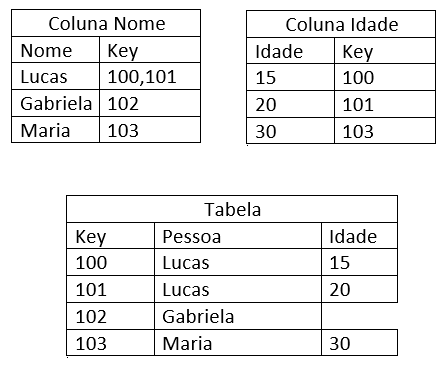
\includegraphics[width=0.4\textwidth]{./04-figuras/db-colunar}
    \fonte{O Autor}
    \label{fig:db-colunar}
\end{figure}


Cada modelo de dados possui suas vantagens e desvantagens, e a melhor escolha depende do que 
se deseja alcançar. Apesar das modelagens e SGBDs não relacionais possuirem claras vantagens,  
elas ainda possuem certas limitações. Por exemplo, a maioria das implementações NoSQL não
suportam as operações \textit{join} e \textit{order by} \cite{pokorny2013nosql}. 
Nesse contexto surgem outras plataformas, para auxiliar no processamento de grandes volumes 
de dados, e que possuem uma comunicação natural com bancos de dados NoSQL. Na próxima seção 
são apresentadas duas dessas plataformas, o Hadoop e o Spark.

\section{Hadoop e Spark}
\label{sec:spark}

O Apache Hadoop\footnote{http://hadoop.apache.org/}, também conhecido apenas como Hadoop, 
é um projeto de código aberto mantido pela Apache Software Foundation, que desenvolve 
softwares para processamento distribuído de grandes volumes de dados. O ecossistema do 
Hadoop é composto por quatro módulos:(1) \textit{Hadoop Common}, (2) 
\textit{Hadoop Distributed File System (HDFS)}, (3) \textit{Hadoop YARN} e (4) 
\textit{Hadoop Map Reduce} \cite{kumar2014apache}. 

O primeiro, \textit{Hadoop Common}, é um conjunto de utilitários que suporta os outros módulos
do Hadoop. O HDFS é um sistema de arquivos distribuído que permite o armazenamento de um 
grande volume de dados em diversos nodos de um \textit{cluster}. As grandes vantagens do HDFS 
são: a portabilidade, capacidade de armazenamento, o custo-benefício e a tolerância a falhas 
\cite{kumar2014apache}.

O YARN é um \textit{framework} para agendamento de tarefas e gerenciamento de recursos em 
\textit{cluster}. Por fim, o \textit{Hadoop MapReduce} é um método para distribuir tarefas 
em múltiplos nodos, o que permite o processamento paralelo e distribuído, tolerante a 
falhas e de fácil abstração. Como o próprio nome sugere, ele é baseado no \textit{MapReduce}, 
um modelo de programação e \textit{framework} introduzido pelo Google \cite{kumar2014apache}. 
A grande desvantagem do Hadoop é que seu processamento ocorre em disco, o que limita sua 
velocidade \cite{shoro2015big}.

Já o Apache Spark\footnote{http://spark.apache.org/}, ou simplesmente Spark, é uma ferramenta 
de propósito geral para processamento em \textit{cluster}, que realiza operações em memória. 
Esta característica permite o aceleramento da análise de dados, tornando mais rápido, 
tanto as operações de escrita quanto o processamento de dados. Em alguns casos o Spark pode ser 
até cem vezes mais rápido que o Hadoop. 

Além disso, o Spark possui APIs para diversas linguagens de programação, como Python, Java, 
Scala e R. Outra vantagem, é a existência de diversas ferramentas de alto nível que auxiliam 
no processamento de dados, como por exemplo a M Lib, uma biblioteca para aprendizado de 
máquina e o Spark SQL, uma biblioteca que permite, entre outras coisas, a realização de 
operações como \textit{join} e \textit{order by} em qualquer conjunto de dados, mesmo 
aqueles originários de bancos de dados NoSQL \cite{shoro2015big}.

Assim, dada uma fonte de dados NoSQL é possível utilizar o Hadoop ou Spark para acessar,
processar e até mesmo alimentar essa fonte. Por fim, deve-se permitir o acesso aos dados
já processados que são armazenados, isso pode ser realizado utilizando \textit{web services}. 


\section{\textit{Web Services}}
\label{sec:api}

A troca de informações entre aplicações distribuídas na web é feita através de protocolos de 
comunicação \cite{schepke2010avaliaccao}. Estes protocolos permitem, entre outras operações, a 
recuperação de dados de aplicações que possuem esse acesso liberado. Serão discutidos duas 
das formas de comunicação, conhecidas como \textit{web services}, mais utilizadas, o 
\textit{Simple Object Access Protocol (SOAP)}, e o \textit{Representational State 
Transfer (REST)} \cite{lima2012}.

O SOAP é um protocolo adotado pela W3C, que permite invocar aplicações remotas independente de 
linguagem de programação e plataforma. O protocolo é baseado em XML, e utiliza o 
\textit{Hypertext Transfer Protocol (HTTP)} para transporte da mensagem. Uma mensagem SOAP é 
composta por três elementos: (1) envelope, (2) cabeçalho e (3) corpo \cite{suda2003soap}.

O envelope SOAP é o recipiente que armazena os outros elementos da mensagem, como o cabeçalho 
e o corpo.  O cabeçalho é um elemento opcional, que contém informações adicionais, como por 
exemplo, se a mensagem deve ser processada por um nó intermediário antes de chegar ao ponto 
final da aplicação. O corpo SOAP é um elemento obrigatório, que armazena os dados da mensagem 
transportada. No caso de uma mensagem de requisição, o corpo pode conter o método a ser 
chamado e os parâmetros de entrada e saída do método, já para uma mensagem de resposta o 
corpo contém o resultado (dados), gerado pelo método chamado \cite{suda2003soap}.

O modelo REST foi definido por \citeonline{fielding2000architectural}, que buscou as melhores 
práticas de arquiteturas de \textit{web services} já existentes e compôs uma nova arquitetura 
que as reunissem em apenas uma. Essa arquitetura reúne as melhores práticas no que se refere 
a: (1) cliente/servidor, (2) sistemas de camadas, (3) cache e (4) sem estado 
\cite{fielding2000architectural}.

No modelo REST são definidos dois papéis, cliente e servidor. O servidor oferece uma série 
de serviços do qual o cliente faz uso. Ao receber uma requisição do cliente o servidor decide 
o que fazer com ela, aceitar a requisição ou rejeitá-la \cite{fielding2000architectural}.

Outra característica do modelo REST é a divisão em camadas. O sistema é dividido de forma que 
uma camada inferior conhece apenas a interface da camada superior, isso melhora a 
escalabilidade do sistema, mas adiciona uma sobrecarga no tratamento dos dados, o que pode 
ser combatido utilizando cache \cite{fielding2000architectural}. 

O cache evita que dados, que já tenham sido enviados anteriormente, sejam reenviados, isso 
melhora a eficiência, escalabilidade e performance dos servidores. Finalmente, o sistema 
não possui estado, ou seja, as informações para atender uma requisição estão contidas nela 
mesma \cite{fielding2000architectural}.

Diferentemente do SOAP, os \textit{web services} REST não possuem um formato padrão para envio 
de mensagens, os mais comuns são o JSON e XML. Além disso, a arquitetura REST utiliza o 
protocolo HTTP e seus métodos para manipulação de recursos. O termo recursos se refere a 
qualquer estrutura que pode ser armazenada em um computador. Esses métodos permitem, entre 
outras operações, a exclusão, atualização, inserção e recuperação de recursos \cite{lima2012}.

A desvantagem do serviço SOAP é o uso limitado do protocolo HTTP, já que utilizam um único 
método para realizar múltiplas operações, enquanto serviços REST utilizam todos os métodos 
disponíveis. Outra desvantagem do SOAP é a falta de flexibilidade na definição do formato 
das mensagens. No entanto, embora os serviços REST sejam mais flexíveis isso também pode ser 
um problema, já que em serviços flexíveis a interoperabilidade pode ficar prejudicada. Não 
existe serviço melhor que o outro, a escolha deve ser feita de acordo com o contexto 
\cite{lima2012}.     % Fundamentação teórica
% -----------------------------------------------------------------------------
% Trabalhos Relacionados
% -----------------------------------------------------------------------------

\chapter{Trabalhos Relacionados}
\label{chap:trabRelac}

Na literatura são encontrados trabalhos referentes a arquitetura de sistemas de visualização,
integração e análise de dados, no contexto dos DGA.  Por exemplo, \citeonline{graves2013} 
mostram como o uso de visualizações podem beneficiar a população, que não possui conhecimento 
técnico, no contexto de DGA. Além disso, os autores demonstram a necessidade de criar 
mecanismos de exploração para navegar por dados e metadados, e quais as funcionalidades uma 
ferramenta deve contemplar para facilitar a criação de visualizações.

Para isso são relatadas três fases em que problemas relacionados a visualizações aparecem, 
como tratar esses problemas, e a apresentação de um protótipo que os resolvem. A primeira fase 
é a de criação, quando ocorre o processamento dos dados que serão usados. Nessa fase deve-se 
resolver questões sobre como tratar dados em formatos diversos, e como combinar dados de 
diferentes bases. A segunda é a fase de exploração, o maior problema nessa fase é a falta de 
informação que garante a qualidade da visualização, como a origem dos dados e o histórico de 
alterações feitas no conjunto de interesse. A última é a fase de adaptar a visualização para 
gerar outros conhecimentos. Nessa fase, devem ser tratados problemas referentes a capacidade 
de modificação dos dados implícitos na visualização, por exemplo, utilizar a média de uma 
métrica no lugar da mediana \cite{graves2013}.

O protótipo proposto por \citeonline{graves2013} utiliza os princípios de \textit{linked data}, 
para integrar os dados e torná-los legíveis tanto para humanos quanto para máquinas. Além 
disso, possui uma interface gráfica que permite a criação de visualizações.

Também seguindo os princípios de \textit{linked data}, \citeonline{hoxha2011open}, propõem a 
utilização de  tecnologias da web semântica para realizar a integração entre dados de 
diferentes organizações governamentais. Os autores propõem uma abordagem composta por três 
módulos, o primeiro é responsável por modelar uma ontologia e converter os dados não 
processados, utilizando o formato do RDF. O segundo é uma interface para consulta a essa base 
de conhecimento, composto por uma interface gráfica e mecanismo para consultas utilizando o 
\textit{Sparql Protocol and RDF Query Language} (SPARQL). O terceiro módulo é uma ferramenta 
de visualização, que faz uso dessa interface de consulta.  Finalmente, os autores sugerem uma 
implementação composta por quatro etapas: processamento dos dados, agregação da informação, 
visualização gráfica e contribuição da comunidade.

Assim como os trabalhos anteriores, \citeonline{ding2010data}, vêm trabalhando em uma 
iniciativa para integrar os dados do Data.gov\footnote{ http://www.data.gov/} (página web 
mantida pelo governo dos Estados Unidos da América, no qual dados referentes ao governo são 
disponibilizados) utilizando os princípios de \textit{linked data}. Os autores mostram como 
as tecnologias de web semântica são utilizadas para converter e integrar esses dados. Para 
isso quatro problemas são tratados: (1) como tornar os dados capazes de fazer parte da 
nuvem do \textit{linked data}, (2) como conectar esses dados entre si e com fontes externas, 
(3) como tornar esses dados utilizáveis para usuários e desenvolvedores e (4) como preservar 
o histórico de dados \cite{ding2010data}.

A solução apresentada por \citeonline{ding2010data} começa tratando das transformações 
necessárias para adequar os dados, isso é feito através da conversão para o formato RDF. 
Após isso, os dados são enriquecidos através de processos semiautomáticos, no qual os valores 
semânticos são associados a URIs que possuem relevância, para isso é utilizado o Semantic 
MediaWiki, que permite que usuários colaborem na edição de conteúdos semânticos. Esses dados 
são disponibilizados através de um \textit{webservice} SPARQL, que permite a integração dos 
dados com APIs convencionais, como a Google Visualization API. Por fim é discutida a 
importância de metadados, que devem permitir avaliar o histórico dos dados, desde sua origem 
até qualquer modificação realizada até o presente.

Fora do contexto dos DGAs também existem trabalhos que tratam da arquitetura de sistemas de 
visualização. \citeonline{viegas2007} discutem o desenho e desenvolvimento do ManyEyes, um 
\textit{website} no qual usuários podem enviar dados, criar visualizações interativas e 
discutir tais visualizações. O objetivo é permitir a colaboração e análise de dados de forma 
social.

Segundo os autores, as decisões de design envolvem três aspectos; (1) a visualização da 
informação, (2) a coleta de dados e manipulação por parte dos usuários, e (3) a colaboração 
de forma social. O site incentiva os usuários a disponibilizarem os metadados e oferece 
suporte para dados no formato de tabelas e texto não estruturado \cite{viegas2007}. 
Por fim os autores discutem os tipos de visualização disponibilizados, como é feito o 
mapeamento dos dados para as visualizações, e os aspectos sociais da ferramenta.

Trabalhos como o realizado por \citeonline{tang2004}, abordam decisões de projeto, para a 
arquitetura de sistemas de visualização de dados. Para isso, \citeonline{tang2004} discutem 
os desafios enfrentados no contexto do Rivet\footnote{https://graphics.stanford.edu/projects/rivet/}, 
um ambiente para desenvolvimento de visualizações. Inicialmente são discutidos três aspectos 
fundamentais: (1) o modelo de dados, (2) a forma de envio, ou seja, como os dados podem ser 
importados para a ferramenta, e (3) as capacidades de transformação que devem existir. 

Em relação ao modelo de dados é discutido as vantagens e desvantagens do modelo relacional, 
comumente utilizado na implementação de sistemas. Para a forma de envio, os autores discutem 
a importância de qualquer dado importado parecer igualmente expressivo para os usuários, ou 
seja, independente do formato a informação armazenada deve ser a mesma. Para isso eles 
disponibilizam diversas formas de se importar dados, passando por conversores CSV até 
drivers para conexão com banco de dados SQL. Quando discutindo os tipos de transformação, 
os autores mostram algumas opções que parecem ser comuns no processo de análise, e, 
portanto, essenciais em um sistema de visualização, como agregação e contagem, ordenação e 
filtros \cite{tang2004}. Além desses aspectos também são tratadas questões como a 
importância de metadados, a modularização na arquitetura e pôr fim a forma de especificação 
para gerar as visualizações.

Para melhor compreender as ferramentas apresentadas, o Quadro \ref{quadro:comparativo} sintetiza as principais 
características das mesmas.

\begin{quadro}[!htb]
    \centering
    \caption{Comparação entre os sistemas encontrados na literatura}
    \label{quadro:comparativo}
    \begin{tabular}{|p{2cm}|p{2cm}|p{2cm}|p{2cm}|p{2cm}|p{2cm}|p{2cm}|}
        \hline
Referência & Modelo de Dados                & Forma de acesso aos dados            & Formato de importação dos dados                   & Importação de dados por usuários & Atualização colaborativa da base de dados & Disponibili- zação de metadados \\
        \hline
\citeonline{graves2013}          & Linked Data                    & Interface gráfica                    & Não especificado                                  & Não especificado                 & Não especificado                          & Sim                           \\
        \hline          
\citeonline{hoxha2011open}         & Linked Data                    & Interface gráfica e consultas SPARQL & Diferentes formatos (XML, CSV, texto)             & Não                              & Não                                       & Sim                           \\
        \hline
\citeonline{ding2010data}          & Linked Data                    & Webservice SPARQL                    & CSV                                               & Não                              & Não                                       & Sim                           \\
        \hline
\citeonline{viegas2007}         & Tabela e texto não estruturado & Interface gráfica                    & Texto separado por tabulação.                     & Sim                              & Não                                       & Sim                           \\
        \hline
\citeonline{tang2004}         & Relacional                     & API REST                             & CSV, MDX e conexões direta com banco de dados SQL & Sim                              & Não                                       & Sim                           \\
        \hline   
    \end{tabular}
    \fonte{O Autor}
\end{quadro}

Embora os trabalhos apresentados contemplem informações sobre a infraestrutura que suporta 
os sistemas de visualização de dados, os autores não detalham os projetos das arquiteturas. 
Também é possível notar que, embora enalteçam a importância do aspecto social na análise de 
dados governamentais abertos, não propõem alternativas concretas que permitam a colaboração 
nas fases mais elementares do processo de análise, por exemplo, durante a inserção ou o 
gerenciamento dos dados.

A ferramenta aqui proposta busca dar suporte a sistemas de visualização colaborativos, e 
estender a capacidade de colaboração para além da geração e análise de visualizações. Ou 
seja, permitir, de forma colaborativa, o processamento e integração de dados distribuídos, 
e estabelecer relacionamento entre esses dados.    % Trabalhos relacionados
% -----------------------------------------------------------------------------
% Metodologia
% -----------------------------------------------------------------------------

\chapter{Metodologia}
\label{chap:metodologia}

A metodologia utilizada na realização desse trabalho consiste em 6 etapas, 
como mostrado na Figura \ref{fig:metodologia}.

\begin{figure}[!htb]
    \centering
    \caption{Metodologia utilizada no trabalho}
    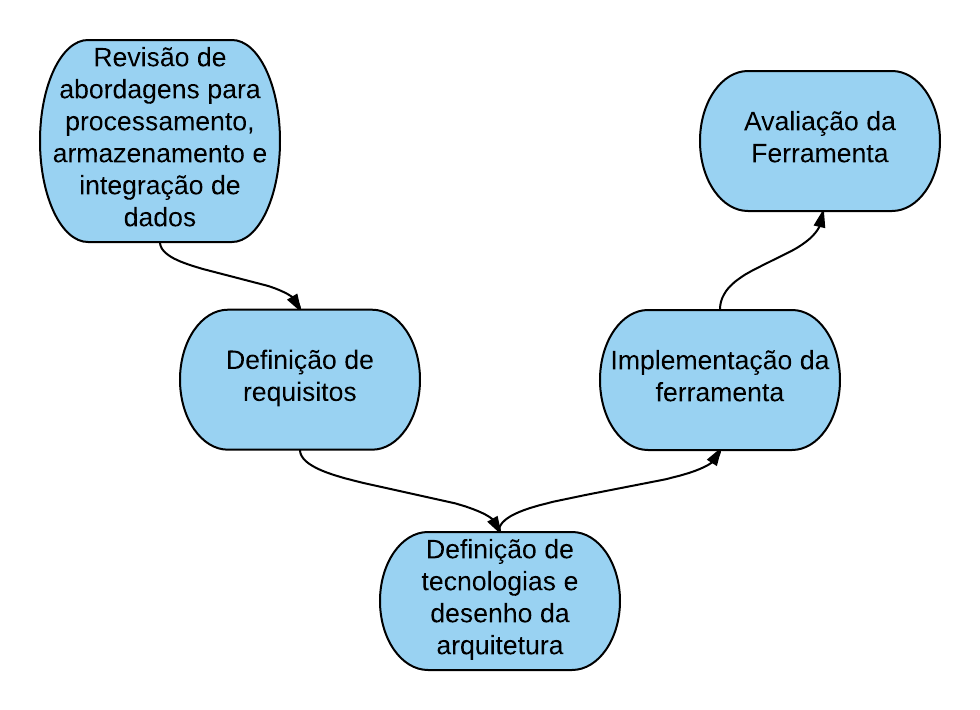
\includegraphics[width=1\textwidth]{./04-figuras/metodologia}
    \fonte{O Autor}
    \label{fig:metodologia}
\end{figure}


Como demonstrado na Figura \ref{fig:metodologia}, o primeiro passo da metodologia consistiu 
em revisar abordagens já existentes para o processamento, armazenamento e integração de dados abertos. 
Essa etapa levantou quais as melhores práticas e alternativas a serem aplicadas no contexto dos 
DGAs. Para isso foi realizado a revisão da literatura acerca do tema, o que deu origem ao 
capitulo \ref{chap:trabRelac}.

A segunda etapa consistiu no levantamento dos requisitos funcionais e não funcionais da 
ferramenta, com o objetivo de delimitar o escopo da mesma. Para isso foi realizada uma reunião,
com especialistas na área, e também foi levado em consideração a revisão da literatura 
feita no passo anterior. Como produto dessa etapa foi gerado um \textit{backlog} com as 
funcionalidades definidas.

A partir dos requisitos levantados anteriormente, foram definidas as tecnologias e o desenho 
da arquitetura que possibilitaram o desenvolvimento da ferramenta. Nesse processo se destaca 
a definição do modelo de dados, a forma de acesso e importação dos dados, e quais tipos de 
metadados seriam especificados pelos usuários. Isso foi feito com base na revisão das 
abordagens, realizada no primeiro passo. Após a definição dos requisitos, das tecnologias e 
feito o desenho da arquitetura, foi realizada a implementação da ferramenta.

Com o término do desenvolvimento a ferramenta foi avaliada segundo a perspectiva do usuário,
através de um Teste de Usabilidade \cite{barbosa2010}. Essa análise traçou as vantagens e 
limitações da ferramenta proposta a partir desse ponto de vista.
               % Metodologia
\chapter{Desenvolvimento}
\label{chap:desenvolvimento}

Neste capítulo, serão apresentadas todas as etapas referentes ao desenvolvimento da ferramenta
WikiOlapBase (WOB), que permite a integração de dados abertos de forma colaborativa. Na seção
\ref{sec:requisitos}, serão explicitados os requisitos levantados para a ferramenta. 
Posteriormente, na seção \ref{sec:arquitetura}, será mostrada a arquitetura proposta para o 
WOB. Finalmente, na seção \ref{sec:wob}, a ferramenta será apresentada, ainda nessa seção será 
apresentada uma análise comparativa entre o WOB e as ferramentas encontradas na literatura.

\section{Levantamento de Requisitos}
\label{sec:requisitos}

Na etapa de Levantamento de Requisitos, foram definidas as funcionalidades e características 
do software proposto. Esse levantamento ocorreu a partir da revisão da literatura e através 
de uma reunião de \textit{brainstorming}, no dia 29 de abril de 2016, com três especialistas 
que possuem mais de oito anos de experiência na área de processamento e análise de dados. 
O resultado gerado foi a lista de requisitos, mostrada no Quadro \ref{quadro:requisitos}.

\begin{quadro}[!htb]
    \centering
    \caption{Requisitos do WOB}
    \label{quadro:requisitos}
    \begin{tabular}{|p{2cm}|p{13cm}|}
        \hline
        Identificador   &   Requisito \\
        \hline
        RF\_1    &  A ferramenta deve permitir a importação de dados, de forma a manter o significado dos dados originais \\   
        \hline
        RF\_2    &  A ferramenta deve ser capaz de converter diferentes formatos para o modelo de dados definido. \\        
        \hline
        RF\_3    &  A ferramenta deve permitir aos usuários o acesso aos dados presentes no banco de dados integrado da ferramenta. \\
        \hline
        RF\_4    &  A ferramenta deve permitir a definição de metadados que se relacionam com um determinado conjunto de dados. \\
        \hline
        RF\_5    &  A ferramenta deve ser capaz de estabelecer relacionamento entre conjunto de dados diferentes. \\
        \hline
        RF\_6    &  A ferramenta deve aceitar arquivos compactados \\
        \hline
        RF\_7    &  A ferramenta deve possibilitar a divisão dos conjuntos de dados em múltiplos arquivos para envio. \\        
        \hline
        RF\_8    &  A ferramenta deve disponibilizar uma interface para que outras aplicações acessem os dados presentes na base de dados integrada. \\
        \hline
        RNF\_1    &  A ferramenta deve ser capaz de armazenar dados em larga escala \\
        \hline
        RNF\_2    &  A ferramenta deve otimizar o tempo de consulta aos dados. \\ 
        \hline   
    \end{tabular}
    \fonte{O Autor}
\end{quadro}

A partir dos requisitos levantados, foi possível escolher as tecnologias, bem como propor uma 
arquitetura, para o desenvolvimento da solução. Na seção a seguir, essas escolhas são expostas 
e justificadas.

\section{Arquitetura do WikiOlapBase}
\label{sec:arquitetura}

A arquitetura do WOB foi especificada de modo a definir: (1) a linguagem de 
programação utilizada, (2) o modelo de dados e os SGBDs utilizados, (3) a forma de acesso 
aos dados, e qualquer outra decisão de projeto. Essas decisões foram tomadas levando em 
consideração a revisão bibliográfica e os requisitos da ferramenta.

Para o desenvolvimento da ferramenta foi utilizado o padrão de arquitetura 
\textit{Model-View-Controller (MVC)}. Nesse padrão, o modelo de dados, a interface do 
usuário e lógica de controle são separados em três componentes: (1) o modelo, que 
representa a estrutura de dados e regras de negócio da aplicação, (2) a \textit{view}, 
que apresenta o modelo para o usuário e (3) o controlador, que interpreta a entrada do 
usuário e se comunica com o modelo para realizar as mudanças necessárias \cite{plekhanova2009evaluating}. 

Essa separação de conceitos, do inglês \textit{separation of concerns (SoC)}, permite o 
desenvolvimento e teste de cada componente de forma independente, o que facilita e agiliza o 
desenvolvimento. Isso também facilita a evolução das funcionalidades de aplicações web, o que 
justifica a escolha do padrão MVC para o desenvolvimento da ferramenta proposta 
\cite{gupta2012}. A Figura \ref{fig:mvc} mostra a interação entre os componentes no 
padrão MVC.

\begin{figure}[!htb]
    \centering
    \caption{Interação entre componentes do MVC}
    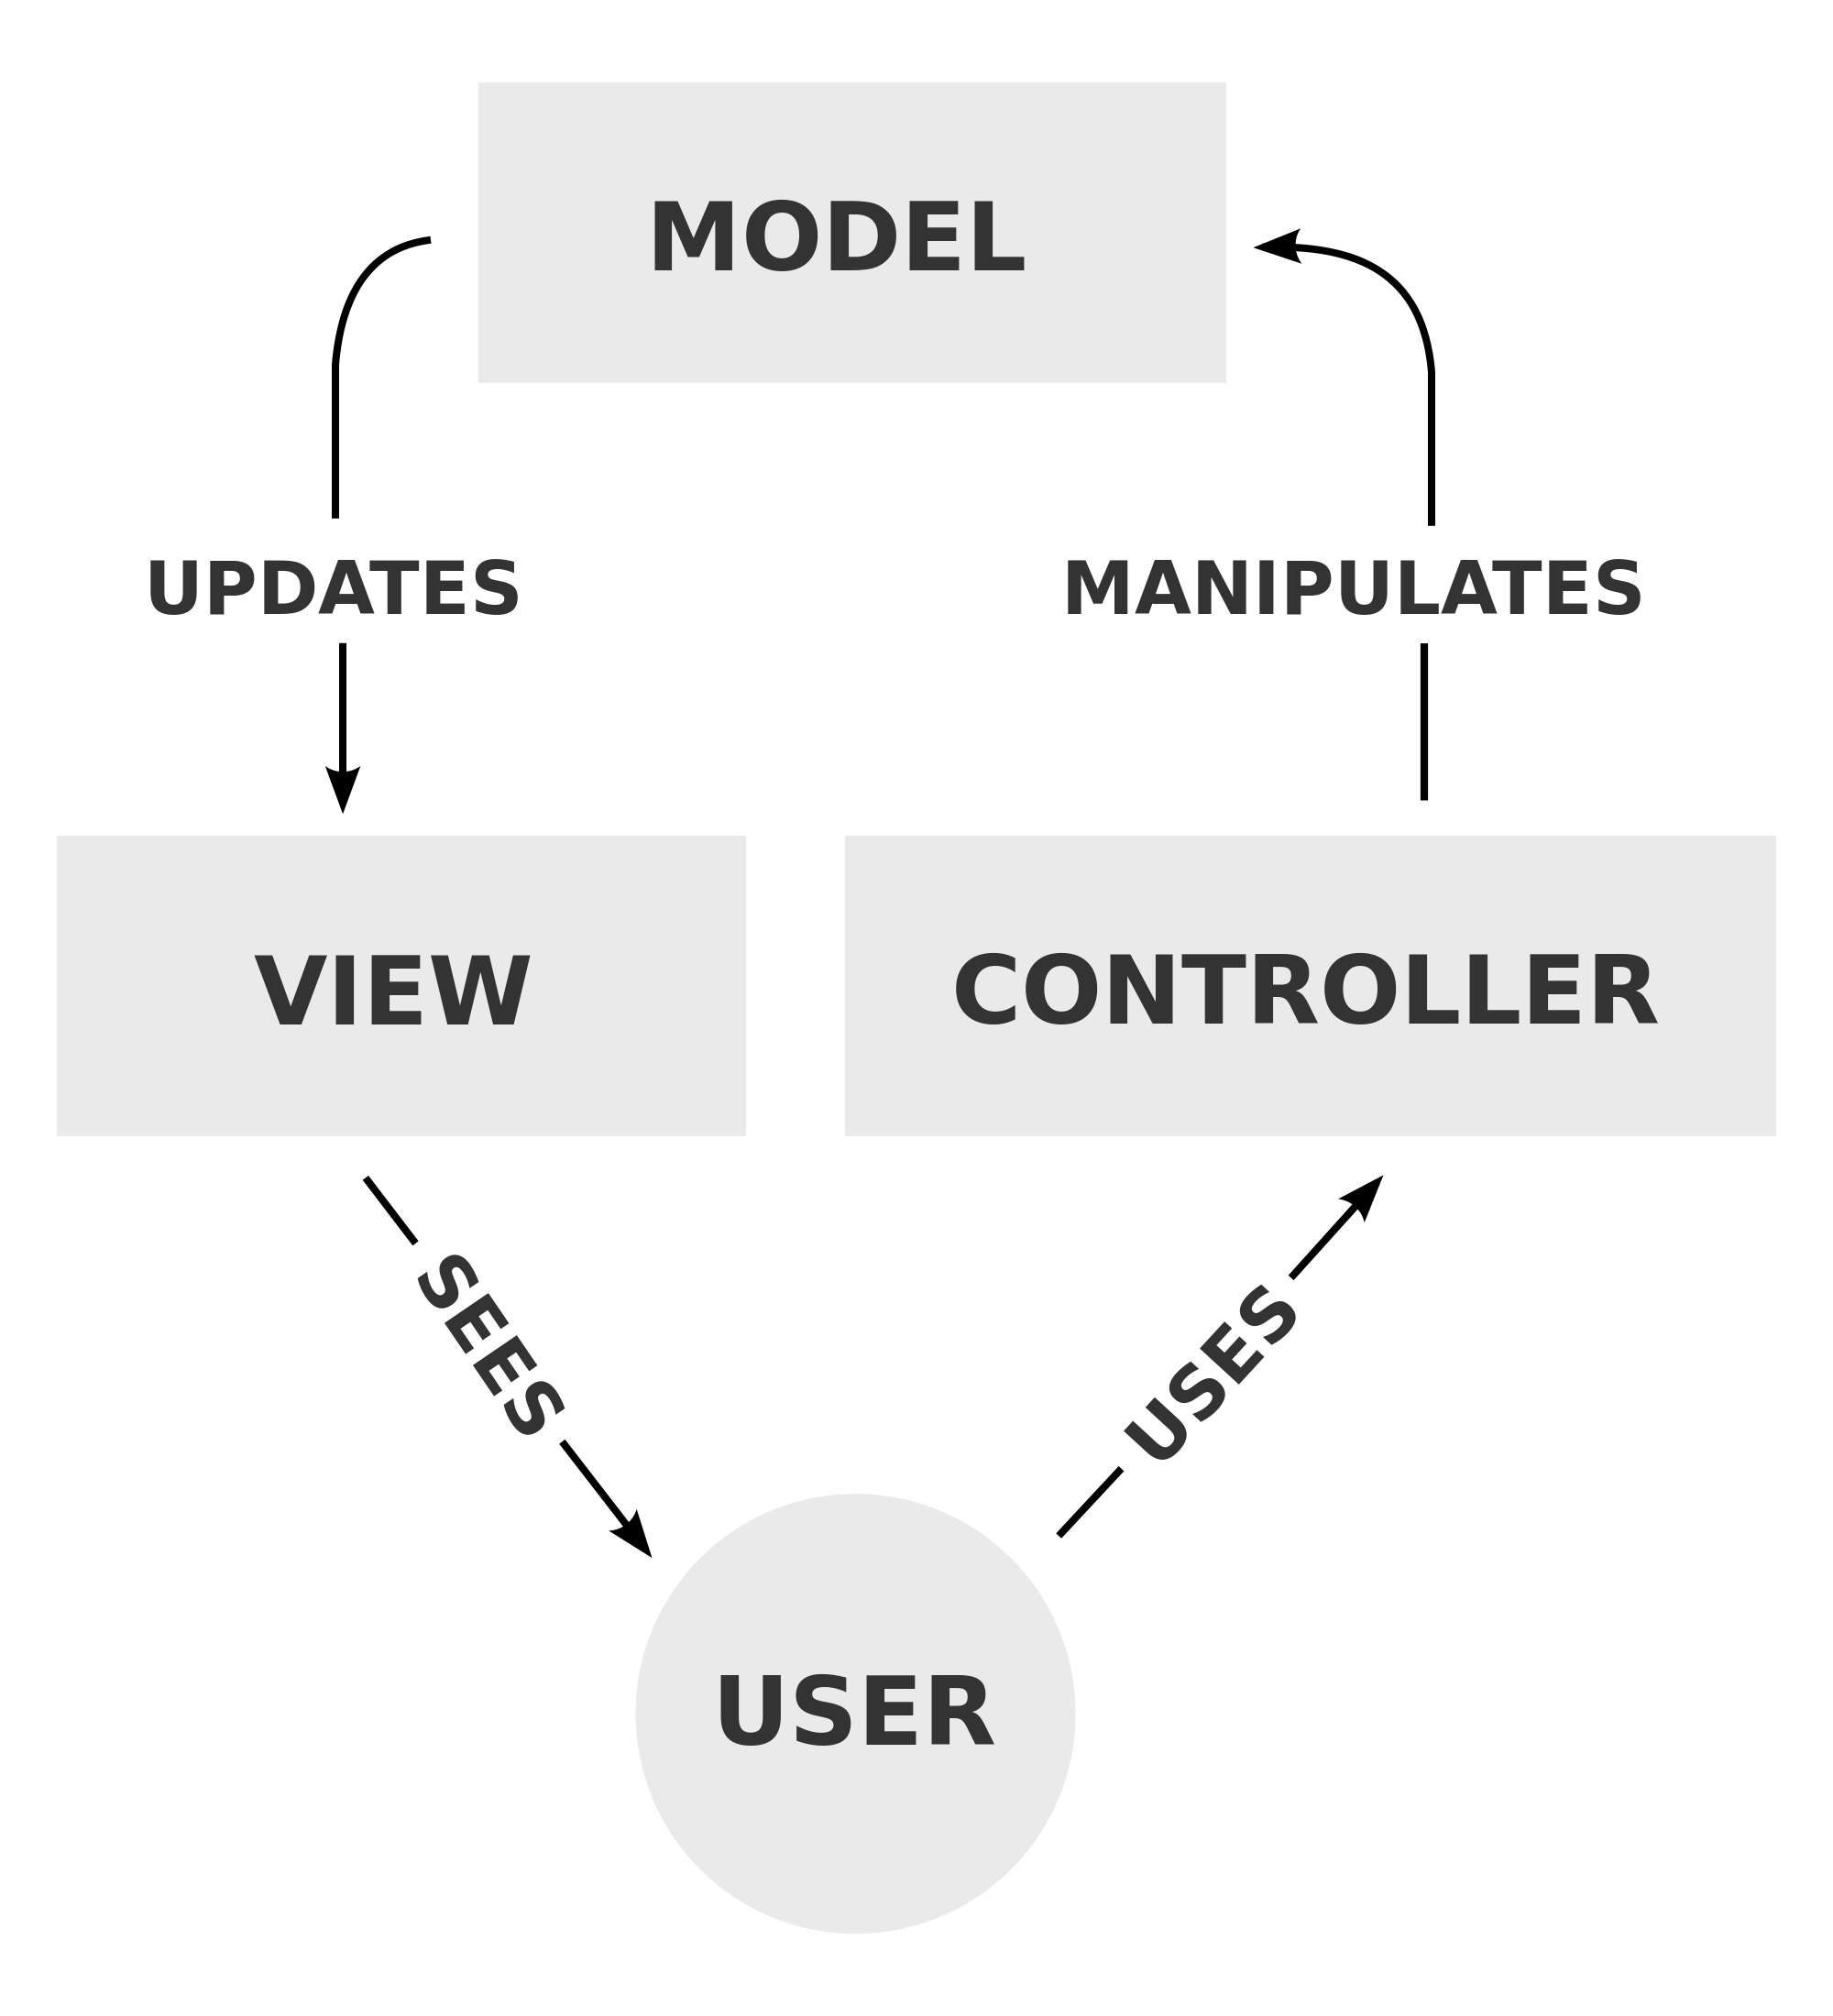
\includegraphics[width=0.4\textwidth]{./04-figuras/mvc}
    \fonte{\citeonline{wiki2016mvc}}
    \label{fig:mvc}
\end{figure}

Para a codificação da ferramenta foi utilizada a linguagem de programação Python, através do 
\textit{framework} Django. Python é uma linguagem de programação popular, que possui suporte 
para integração com outras linguagens e ferramentas, além de uma variedade de bibliotecas. 
Já o Django, é um \textit{framework} de código aberto que busca automatizar ao máximo o 
desenvolvimento, aderindo ao princípio "não repita a si mesmo", do inglês 
\textit{don’t repeat yourself (DRY)} \cite{plekhanova2009evaluating}. Também vale ressaltar 
que para a interface do usuário foram usadas as linguagens 
\textit{HyperText Markup Language} (HTML), \textit{Cascading Style Sheets (CSS)} e JavaScript.

A arquitetura aqui proposta busca funcionar como infraestrutura base para ferramentas de
visualização de grandes volumes de dados que fazem uso de operações OLAP, e portanto, 
o modelo de dados escolhido deve viabilizar isso. Dessa forma, foi escolhido o modelo de 
família de colunas, pois ele otimiza esse tipo de operações, que tipicamente envolvem
consultas complexas em grandes porções de dados \cite{sorjonen2012olap}. 

Comparativamente, bancos de dados relacionais, orientados por linha, precisam manipular uma 
grande quantidade de itens para selecionar os dados necessários para responder a uma consulta, 
o que torna operações de leitura lentas, e portanto não indicadas quando se deixa realizar 
uma operação OLAP \cite{sorjonen2012olap}. Já bancos de dados orientados por coluna, acessam 
apenas os itens necessários para responder uma consulta, o que torna as operações de leitura
mais rápidas. Além disso, o modelo de família de colunas é mais escalável, o que no contexto
de grandes volumes de dados é uma característica desejada \cite{moniruzzaman2013nosql}.

Além dos conjuntos de dados que serão armazenados pela ferramenta, também foi necessário 
registrar os metadados referentes a esses conjuntos, de modo que seja possível 
caracterizá-los. Metadados são comumente definidos como dados sobre dados. No entanto, vão 
além dessa definição. Eles permitem ao usuário, ou um computador, procurar e gerenciar 
informações, definir as regras para uma estrutura de dados e integrar dados de diferentes 
fontes \cite{turner2002metadata}. Desse modo, para o armazenamento dos metadados, foi 
utilizado o modelo orientado a documentos. Esse modelo não possui 
estrutura definida, o que o torna uma boa escolha para armazenamento de metadados 
\cite{de2010nosql}.

O SGBD utilizado para implementar e gerenciar o modelo de família de colunas foi o 
Cassandra, já o modelo orientado a documentos foi implementado no MongoDB. 
Segundo o site db-engines.com (2016), esses dois SGBDs estão entre os dez mais utilizados, 
sendo os primeiros colocados em suas categorias. Isso demonstra a popularidade e aceitação 
da comunidade em relação a essas ferramentas, o que justifica suas escolhas. Devido às 
limitações dos bancos de dados NoSQL, já explorada anteriormente (na Seção \ref{sec:bigdata}), 
também foi utilizada a plataforma Spark para realizar uma interface com o Cassandra. A 
utilização do Spark permite a realização de operações mais complexas sobre os dados, além de 
tornar ainda mais rápida a leitura e escrita de dados sobre o Cassandra \cite{kolaczkowski2014}.

Finalmente, para o acesso aos dados, foi disponibilizado uma API REST, devido a sua 
simplicidade e adequação natural a web \cite{maleshkova2010}. A Figura \ref{fig:arquitetura} apresenta o 
diagrama da arquitetura implementada.  

\begin{figure}[!htb]
    \centering
    \caption{Arquitetura do WikiOlapBase}
    \includegraphics[width=0.7\textwidth]{./04-figuras/arquitetura}
    \fonte{O Autor}
    \label{fig:arquitetura}
\end{figure}

\section{WikiOlapBase}
\label{sec:wob}

A partir da arquitetura proposta na seção \ref{sec:arquitetura} e nos requisitos definidos
na seção \ref{sec:requisitos} a ferramenta WikiOlapBase foi implementada. O desenvolvimento 
foi iniciado no dia 2 de junho de 2016 e a primeira versão funcional foi finalizada no dia 
22 de setembro de 2016, demorando, portanto, 3 meses e 20 dias.

A ferramenta proposta possui dois módulos: o primeiro é responsável por receber, caracterizar
e integrar os conjuntos de dados enviados pelos usuários, o segundo permite o acesso a esse 
repositório de dados integrados por meio de uma API REST. O primeiro módulo é composto por 
uma série de interfaces, nas quais os usuários preenchem os metadados referente a base de 
dados que está sendo enviada. O conjunto de dados é então processado e armazenado no 
Cassandra, já os metadados são armazenados no MongoDB. 

Para realizar o armazenamento no Cassandra, é utilizada uma API do Spark, o que torna esse 
processo mais rápido e eficaz \cite{kolaczkowski2014}. Já a API REST possui diversos métodos 
que podem ser acessados para realizar operações como: recuperação de dados, recuperação de 
metadados e cruzamento entre diferentes bases de dados. Para que o usuário possa recuperar 
e pré-processar os dados foi utilizada uma API do Spark, que realiza essas operações de uma 
forma mais rápida \cite{kolaczkowski2014}. A seguir serão detalhados os principais passos 
do fluxo de execução da ferramenta.

O fluxo de execução principal do WOB é composto por quatro passos, para facilitar o 
aprendizado do usuário foi elaborada uma interface que explica esses passos, conforme
demonstrado nas Figuras \ref{fig:wob-ajuda}, \ref{fig:wob-ajuda2}, \ref{fig:wob-ajuda3} e
\ref{fig:wob-ajuda4}. A Figura \ref{fig:wob-ajuda} mostra como realizar o primeiro passo de execução 
da ferramenta, quando o arquivo referente ao conjunto de dados é enviado. Em seguida, a 
Figura \ref{fig:wob-ajuda2} mostra como realizar o segundo passo de execução, na qual o
usuário deve preencher informações básicas sobre o conjunto sendo enviado. Já a Figura \ref{fig:wob-ajuda3} 
mostra como executar o terceiro passo de execução, nessa etapa é possível renomear colunas e 
adicionar \textit{tags} a cada coluna. Por fim, a Figura \ref{fig:wob-ajuda4} mostra como 
executar o último passo, na qual é possível adicionar hierarquias de dados ao
conjunto sendo salvo.

\begin{figure}[!htb]
    \centering
    \caption{Interface de instruções do WOB - Passo 1}
    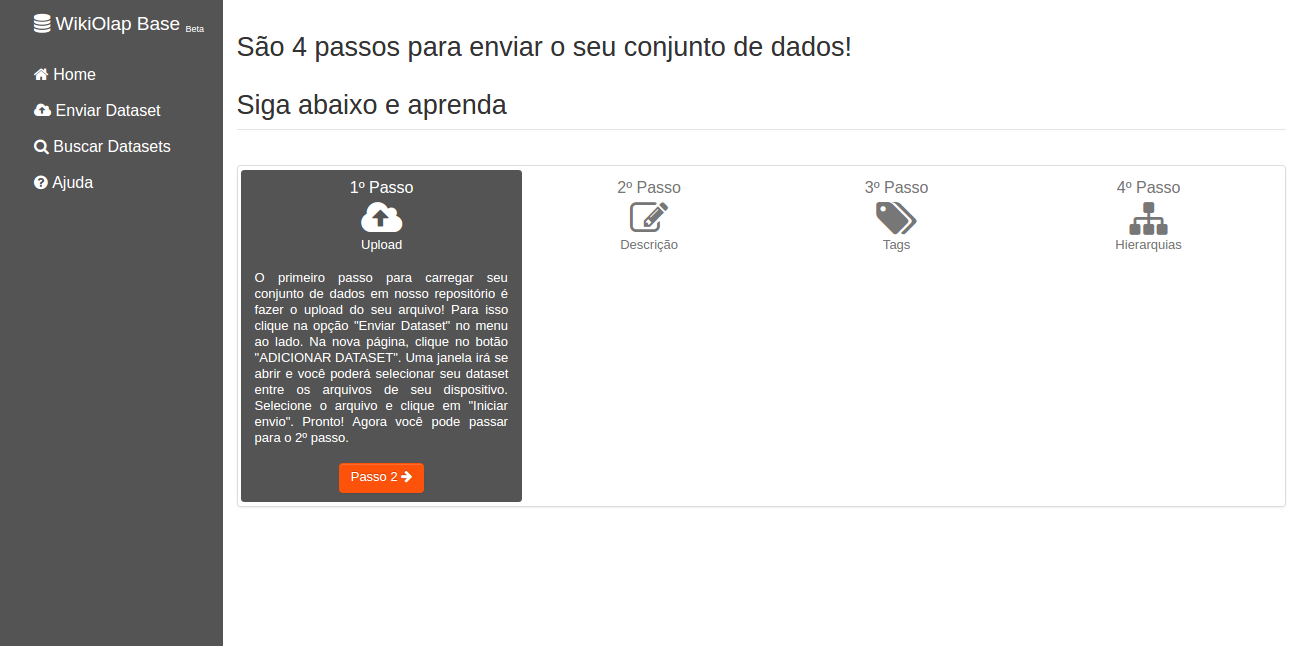
\includegraphics[width=0.7\textwidth]{./04-figuras/wob-ajuda}
    \fonte{O Autor}
    \label{fig:wob-ajuda}
\end{figure}

\begin{figure}[!htb]
    \centering
    \caption{Interface de instruções do WOB - Passo 2}
    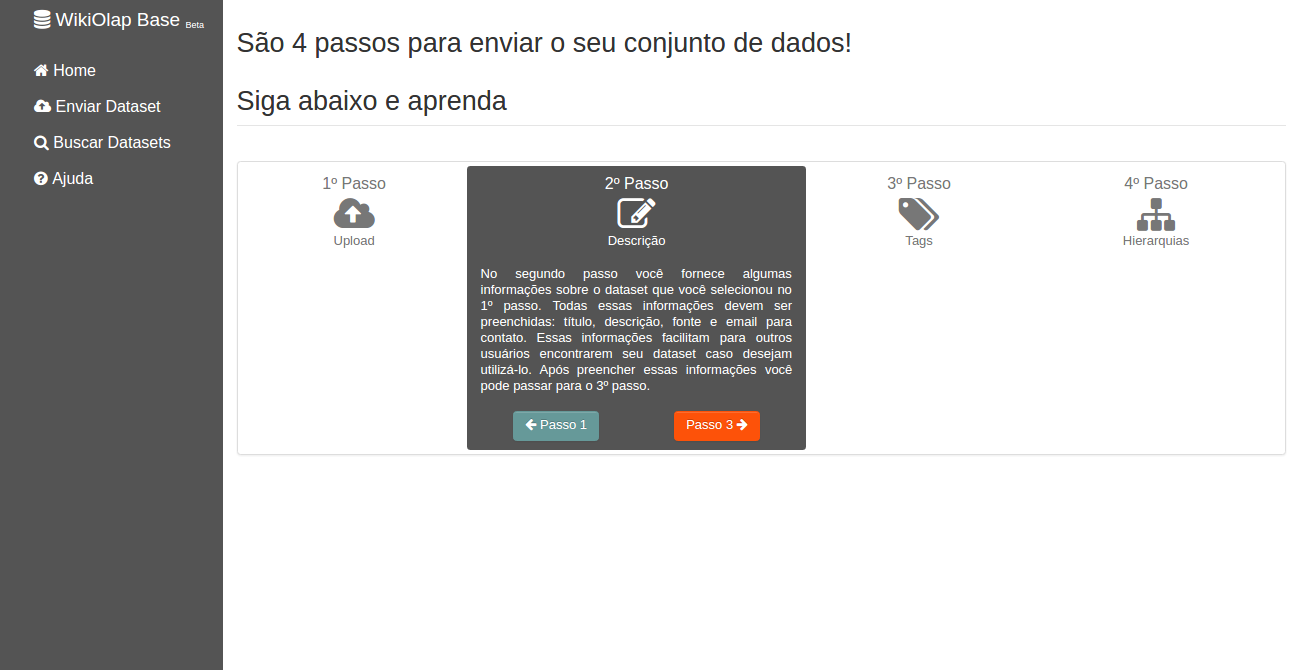
\includegraphics[width=0.7\textwidth]{./04-figuras/wob-ajuda2}
    \fonte{O Autor}
    \label{fig:wob-ajuda2}
\end{figure}

\begin{figure}[!htb]
    \centering
    \caption{Interface de instruções do WOB - Passo 3}
    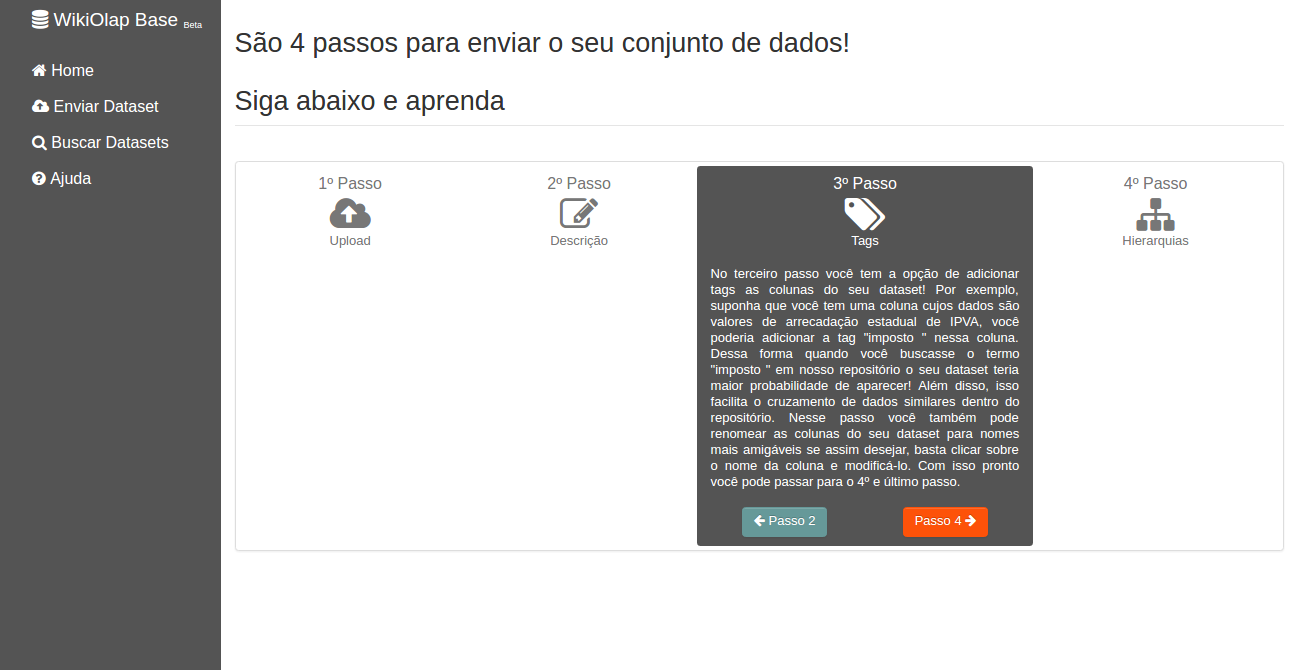
\includegraphics[width=0.7\textwidth]{./04-figuras/wob-ajuda3}
    \fonte{O Autor}
    \label{fig:wob-ajuda3}
\end{figure}

\begin{figure}[!htb]
    \centering
    \caption{Interface de instruções do WOB - Passo 4}
    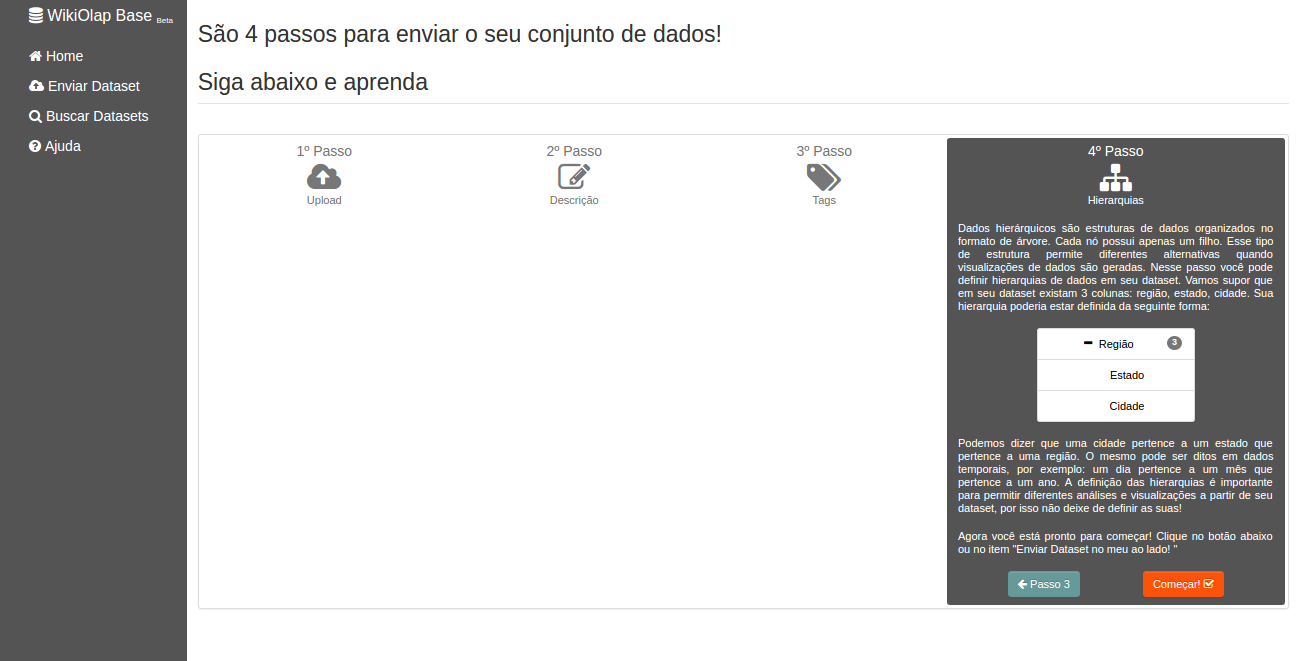
\includegraphics[width=0.7\textwidth]{./04-figuras/wob-ajuda4}
    \fonte{O Autor}
    \label{fig:wob-ajuda4}
\end{figure}

O primeiro passo de execução engloba a seleção e envio do conjunto de dados desejado, vale
ressaltar que nessa primeira versão só são aceitos arquivos no formato CSV, a Figura \ref{fig:wob-sendfile} 
mostra a interface elaborada para essas ações. A partir dos dados enviados o usuário deve 
preencher os metadados correspondentes, esse procedimento engloba os três passos de execução 
seguintes, embora seja sugerida uma sequência, o usuário pode realizar essa fase na ordem 
que desejar. 

\begin{figure}[!htb]
    \centering
    \caption{Interface para envio de arquivo do WOB}
    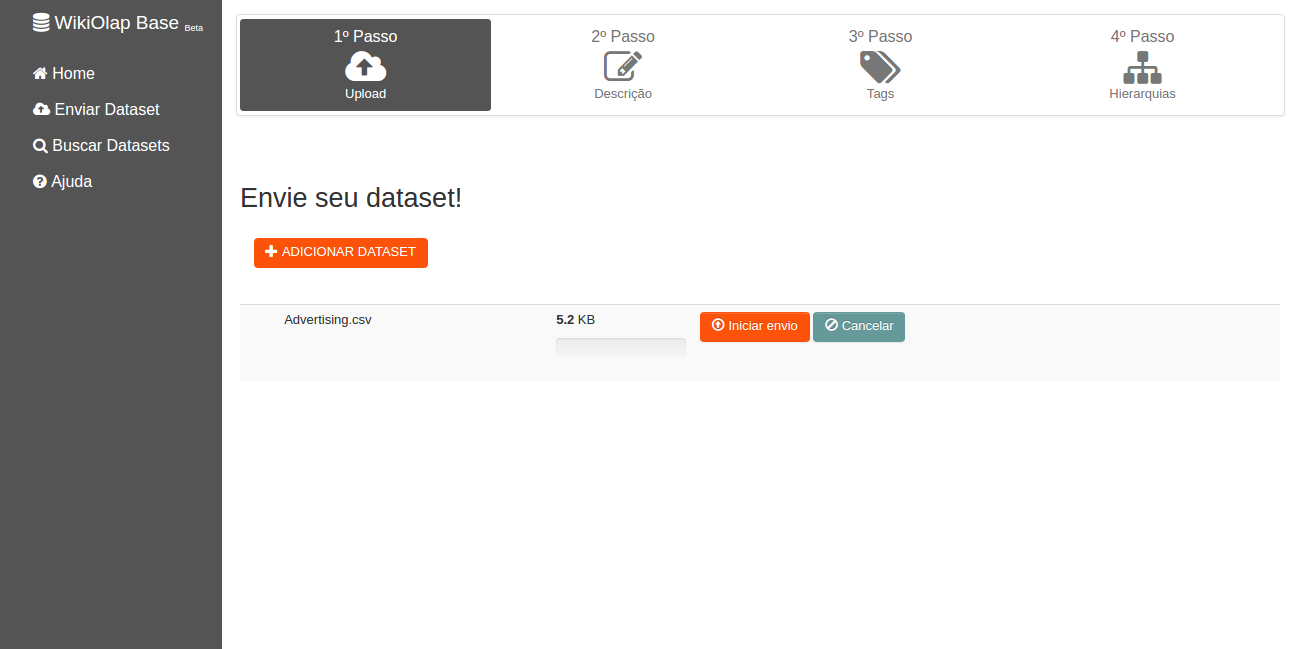
\includegraphics[width=1.1\textwidth]{./04-figuras/wob-sendfile}
    \fonte{O Autor}
    \label{fig:wob-sendfile}
\end{figure}

Seguindo a sequência sugerida, primeiro deve ser preenchido informações básicas do conjunto 
de dados, como fonte, título e descrição. Essas informações permitem a indexação dentro do 
repositório, possibilitando, posteriormente, que outros usuários possam buscar esses dados, 
a interface pode ser vista na Figura \ref{fig:wob-info}.

\begin{figure}[!htb]
    \centering
    \caption{Interface para preenchimento de informações básicas do WOB}
    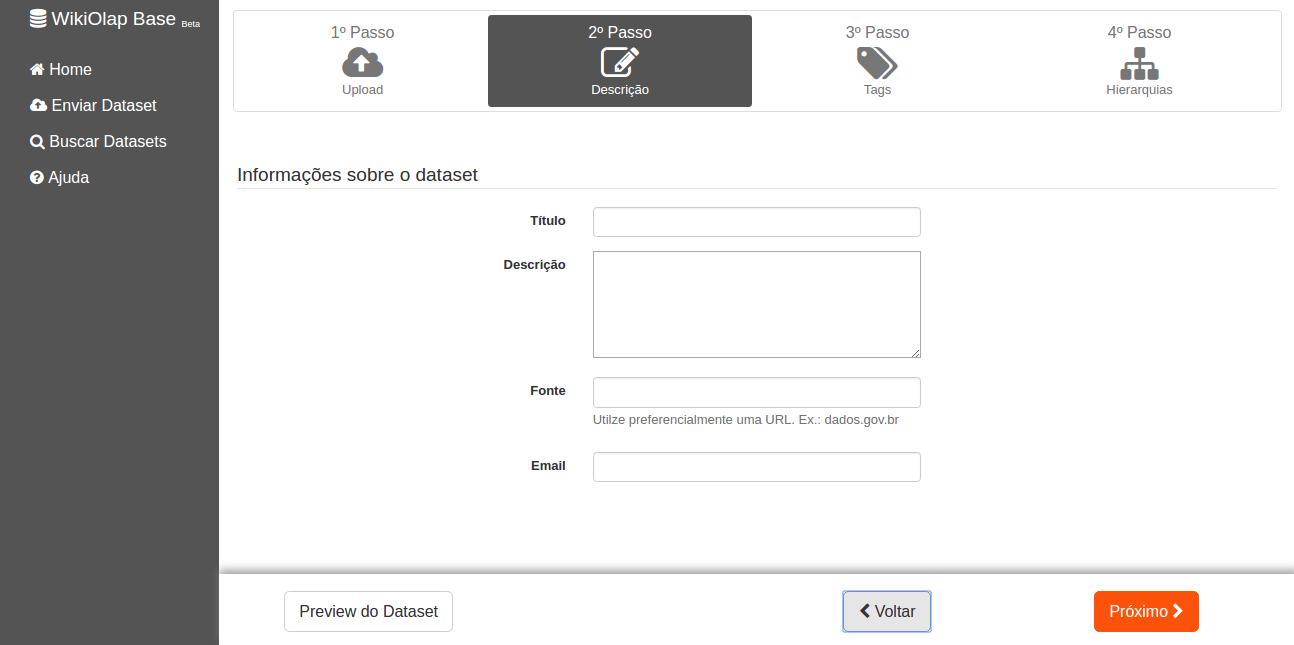
\includegraphics[width=1\textwidth]{./04-figuras/wob-info}
    \fonte{O Autor}
    \label{fig:wob-info}
\end{figure} \newpage


Logo depois, o usuário pode adicionar \textit{tags} às colunas do conjunto de dados. Isso, 
além de ajudar na indexação desses dados, também viabiliza o cruzamento entre conjuntos 
diferentes, pois permite a descoberta de conjuntos de dados que possuem atributos em comum. 
Nesse ponto o usuário também pode renomear as colunas, se assim o desejar, essa interface é 
mostrada na Figura \ref{fig:wob-tags}. 

\begin{figure}[!htb]
    \centering
    \caption{Interface para preenchimento de tags do WOB}
    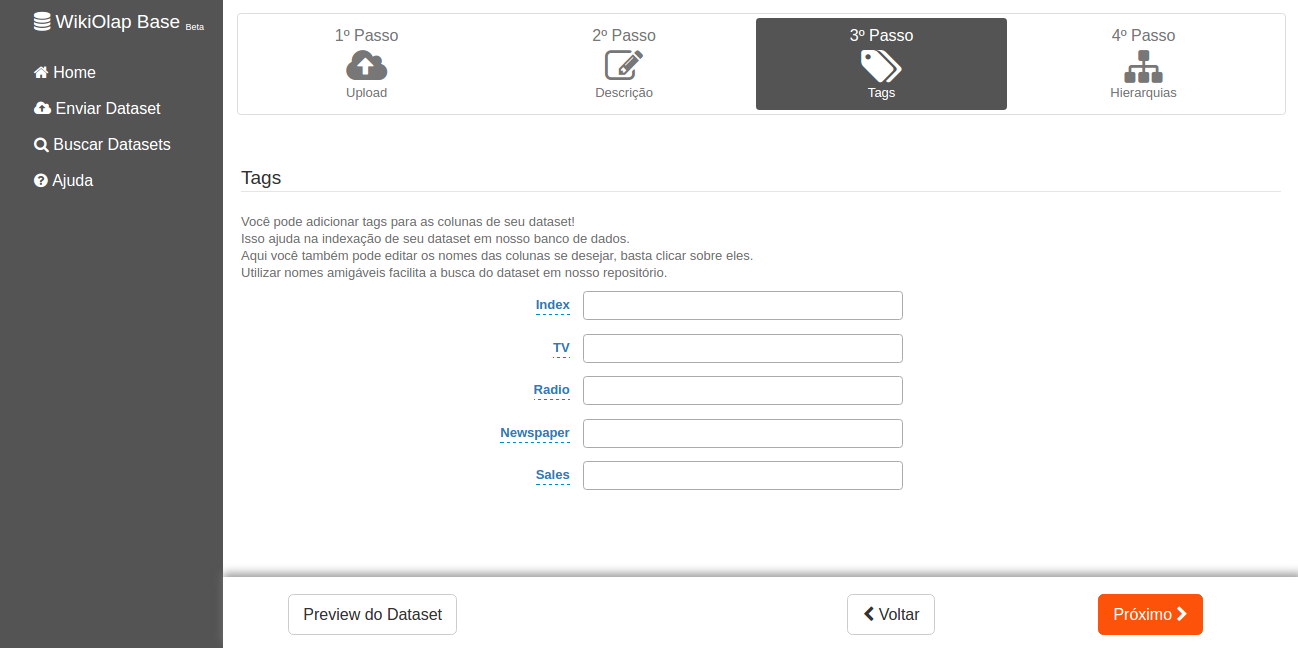
\includegraphics[width=0.9\textwidth]{./04-figuras/wob-tags}
    \fonte{O Autor}
    \label{fig:wob-tags}
\end{figure}

Por fim, o usuário pode identificar hierarquias de dados dentro do conjunto enviado. Essa 
informação pode ser utilizada na geração de visualizações que utilizam operações OLAP como 
\textit{drill down} e \textit{drill up}, a interface pode ser vista na Figura \ref{fig:wob-hierarquia}. 
Além disso também é disponibilizado ao usuário um \textit{preview} de seu conjunto de dados, 
desse modo ele pode verificar se não ocorreu um erro ao enviar seu arquivo.

\begin{figure}[!htb]
    \centering
    \caption{Interface para indentificação de hierarquias do WOB}
    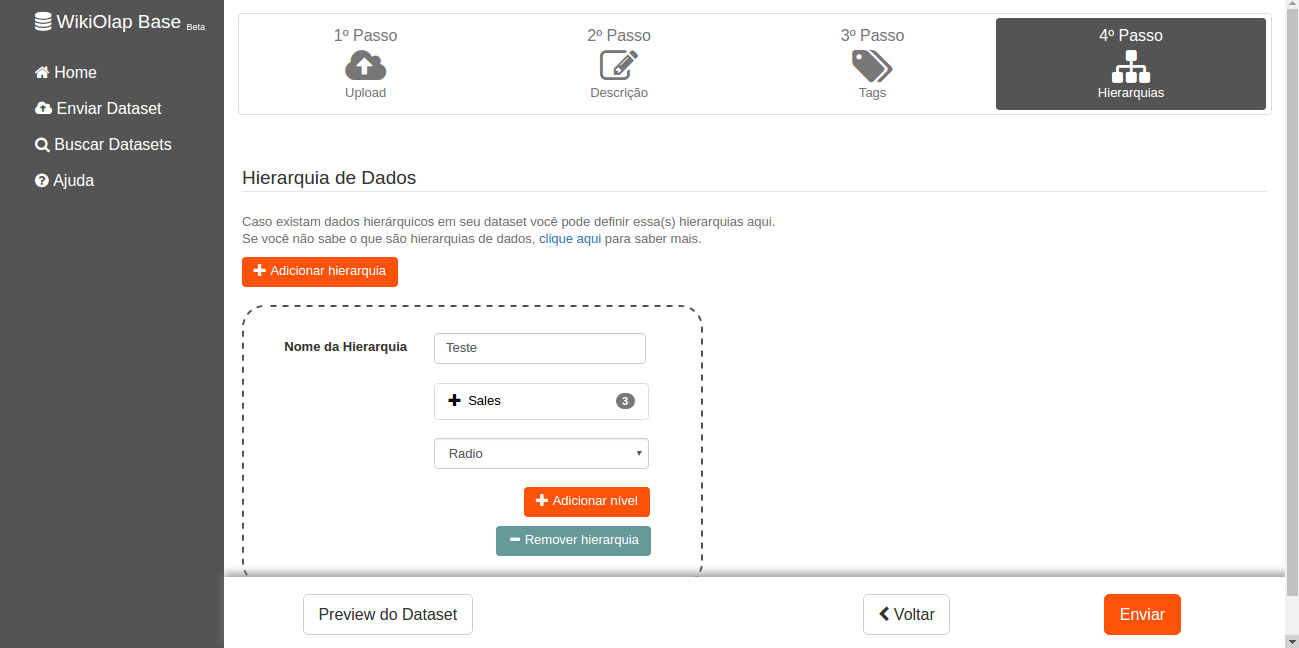
\includegraphics[width=0.85\textwidth]{./04-figuras/wob-hierarquia}
    \fonte{O Autor}
    \label{fig:wob-hierarquia}
\end{figure}

Essa sequência de ações, realizadas pelo usuário da ferramenta, viabiliza a integração entre
o conjunto de dados enviado por ele e os que já existem no repositório. Além disso, o 
preenchimento consciente dos metadados faz parte do aspecto colaborativo da ferramenta, 
já que isso possibilita a reutilização dos conjuntos enviados por qualquer usuário que 
assim o desejar.

Finalmente, para acessar o repositório do WikiOlapBase, e realizar operações em cima dos 
conjuntos de dados disponíveis, os usuários podem utilizar a API REST que foi desenvolvida, 
sua documentação\footnote{http://docs.wikiolapapi.apiary.io/} já se encontra disponível. 
Embora a ferramenta em si ainda não esteja disponível para o público em geral, o código 
fonte\footnote{https://github.com/pedromb/wikiolapbase} já é de domínio público.

Percebe-se que o WikiOlapBase possui algumas características que o diferenciam das outras ferramentas
mostradas no capítulo \ref{chap:trabRelac}. O Quadro \ref{quadro:comparativo2} mostra um 
comparativo entre as ferramentas e o WOB.

\begin{quadro}[!htb]
    \centering
    \caption{Comparação entre os sistemas encontrados na literatura e o WikiOlapBase}
    \label{quadro:comparativo2}
    \begin{tabular}{|p{1.75cm}|p{1.75cm}|p{1.75cm}|p{1.75cm}|p{1.75cm}|p{1.75cm}|p{1.5cm}|p{1.5cm}|}
        \hline
Referência & Modelo de Dados & Forma de acesso aos dados & Formato de importação dos dados & Importa- ção de dados por usuários & Acesso a base de dados de outros usuários & Disponi- bilização de metadados & Cruza- mento entre dados\footnotemark\\
        \hline
OpenData- Vis - \citeonline{graves2013} & Linked Data & Interface gráfica & Não especificado & Não especificado & Não especificado & Sim & Não \\
        \hline          
\citeonline{hoxha2011open} & Linked Data & Interface gráfica e consultas SPARQL & Diferentes formatos (XML, CSV, texto) & Não & Não & Sim & Não \\
        \hline
Data-GovWiki - \citeonline{ding2010data} & Linked Data & Web- service SPARQL & CSV & Não & Não & Sim & Não\\
        \hline
Many Eyes - \citeonline{viegas2007} & Tabela e texto não estruturado & Interface gráfica & Texto separado por tabulação. & Sim & Sim & Sim & Não \\
        \hline
Rivet - \citeonline{tang2004} & Relacional & API REST & CSV, MDX e conexões SQL & Sim & Não & Sim & Não \\
        \hline
WikiOlap- Base & Família de colunas & API REST & CSV & Sim & Sim & Sim & Sim \\
        \hline   
    \end{tabular}
    \fonte{O Autor}
\end{quadro}
\footnotetext{Utilizando dados enviados por outros usuários}

Pode-se observar que o WOB possui dois grandes diferenciais, o primeiro é o aspecto colaborativo,
já que todo gerenciamento da base de dados é feita pelos próprios usuários. O segundo diferencial
é a possibilidade de relacionar conjuntos de dados que estão disponíveis no repositório. 
Já um aspecto a ser melhorado pelo WOB é a disponibilidade de importação de dados em 
diferentes formatos, já que na versão inicial só está disponível o formato CSV.

É possível perceber que dos requisitos levantados na seção \ref{sec:requisitos} nem todos foram
atendidos. No entanto, aqueles que permitem o fluxo de execução básico e tornam a plataforma
funcional foram implementados, são eles: permitir a importação de dados de forma a manter o
significado dos dados originais; converter formatos de arquivos diferentes para o modelo de dados
definido; permitir o acesso aos dados presentes na base integrada; permitir a definição de metadados. 
Já os requisitos não funcionais não foram medidos. No entanto, a arquitetura foi desenhada de modo
a atender tais requisitos.

Após o desenvolvimento da ferramenta foi realizada de uma avaliação de usabilidade,
com o objetivo de determinar se a ferramenta está adequada ao uso por parte do público alvo.
O capítulo seguinte mostra a metodologia utilizada e os resultados alcançados nessa avaliação.           % Desenvolvimento
\chapter{Avaliação do WikiOlapBase}
\label{chap:avaliacao}

Terminado o desenvolvimento do WikiOlapBase foi realizada a avaliação da ferramenta, segundo
a perspectiva dos usuários. Dois fatores são importantes na ferramenta desenvolvida, primeiro 
que ela seja adequada a utilização por parte do público alvo e segundo que ela permita a 
colaboração entre usuários \cite{barbosa2010}. Neste capítulo são discutidos a 
metodologia e os resultados da avaliação do WOB na visão de seus usuários.

\section{Metodologia de Avaliação}
\label{sec:metodologia-avaliacao}

Com intuito de avaliar a adequação de uso da ferramenta WOB, foi realizado um Teste de 
Usabilidade. Este teste consiste em um método de avaliação de interface que, além dos 
avaliadores, envolve a participação de usuários e prevê as seguintes fases: preparação, 
execução e análise \cite{barbosa2010}.

A fase de preparação é subdividida nas etapas de: (1) determinação dos objetivos do teste; 
(2) definição das tarefas que serão executadas; (3) seleção dos participantes; (4) 
considerações sobre os aspectos éticos; e (5) execução do teste piloto. Essas etapas geram 
artefatos que são posteriormente utilizados durante o passo de execução do Teste de 
Usabilidade. Dentre esses artefatos, incluem-se o \textit{Script} para apresentação do sistema, 
os  cenários de descrição das tarefas, o questionário de seleção dos participantes, o 
questionário pré-teste e o formulário de consentimento \cite{barbosa2010}.

É importante ressaltar que, além das tarefas que serão executadas pelos usuários, são 
definidas as métricas de usabilidade que serão observadas em cada execução. Para cada 
medida, são definidos os limites mínimos aceitáveis, os limites máximos possíveis e o 
valor almejado de usabilidade para cada métrica \cite{barbosa2010}.

A execução representa a fase em que ocorre a avaliação do sistema sob a perspectiva dos 
usuários. O avaliador conduz essa fase, efetuando as etapas de: (1) recebimento do usuário; 
(2) apresentação do sistema, conforme o \textit{Script} preparado; (3) consentimento formal 
dos usuários, utilizando para isso o termo de consentimento; (4) questionamento pré-teste, 
utilizando o questionário preparado; (5) observação das tarefas executadas pelos usuários e 
(6) a entrevista ou questionário pós-teste \cite{barbosa2010}.

Já na terceira fase do método, os dados coletados pelo avaliador são analisados. Nessa fase 
ocorre a verificação de cada uma das medidas de usabilidade, observadas durante a fase de 
execução, relacionando-as aos valores almejados durante a preparação. Nesse passo também 
são classificadas as gravidades dos problemas encontrados e possivelmente são discutidas as 
hipóteses relacionadas às causas dos problemas encontrados. Todos estes passos são 
posteriormente relatados em um relatório final do Teste de Usabilidade \cite{barbosa2010}.

Após elucidado a forma de condução do Teste de Usabilidade, é possível relatar como esse 
método foi conduzido para a avaliação da ferramenta WOB. Na fase de preparação, após 
estabelecido o objetivo do teste (i.e., avaliar a usabilidade e os mecanismos de 
colaboração do WOB), foram elaborados os artefatos que seriam utilizados durante as 
avaliações. São eles: o \textit{Script} da avaliação, o termo de consentimento de participação, 
os cenários de descrição das tarefas, a ficha de controle da avaliação e o questionário
referente ao grau de adequação à usabilidade. Esses artefatos podem ser visualizados no 
Apêndice \ref{apendiceA}.

Em relação às tarefas, é importante ressaltar que foram considerados os principais cenários 
de interação com o WOB, conforme segue: (T1) aprender a utilizar a ferramenta a partir das 
instruções presentes na seção de ajuda, (T2) enviar um conjunto de dados no formato CSV, (T3) 
observar o \textit{preview} do conjunto de dados, (T4) preencher as informações básicas referentes ao 
conjunto de dados, (T5) definir \textit{tags} para as colunas do arquivo enviado e 
renomeá-las, (T6) definir uma hierarquia de dados dentro do conjunto enviado, (T7) enviar os 
metadados, (T8) verificar se o conjunto de dados foi incluído no repositório utilizando a 
ferramenta de busca, (T9) utilizar a API disponível para recuperar os dados que foram 
enviados e gerar visualizações e (T10) utilizar a API para cruzar dois conjuntos de 
dados distintos e gerar visualizações. 

A partir dessas tarefas foram definidos três cenários diferentes que envolvem uma ou mais 
delas, da seguinte forma: (C1) que envolve enviar um conjunto de dados e gerar uma 
visualização a partir do mesmo, para isso é necessário realizar as tarefas de T1 a T9; 
(C2) no qual deve-se enviar um conjunto de dados e fazer o cruzamento do mesmo com outro 
conjunto já existente no repositório para gerar uma visualização, para isso é 
preciso realizar as tarefas de T1 a T8, e T10; (C3) que envolve utilizar dois conjuntos de 
dados já existentes no repositório e gerar uma visualização a partir deles, logo é 
necessário realizar as tarefas T8 e T10.

Para a realização dos cenários de avaliação, os usuários utilizaram dois conjuntos de dados de teste.
O primeiro conjunto é referente a série histórica da contribuição provisória sobre movimentações
financeiras (CPMF), e o segundo referente a série histórica do índice nacional de preços ao
consumidor amplo (IPCA), um índice tipicamente ligado aos níveis de inflação. 
Esses dados foram obtidos no \textit{website} do Instituto de Pesquisa Econômica Aplicada 
(IPEA), uma fundação pública federal vinculada ao Ministério do Planejamento, Desenvolvimento e 
Gestão. Esses conjuntos de dados são exemplos de dados abertos que podem ser integrados no 
WikiOlapBase. A Figura \ref{fig:visualizacao} mostra o resultado da execução do cenário C3. 
Nela podemos ver o resultado do cruzamento entre os dois conjuntos de dados utilizados, isso 
permite avaliar, por exemplo, a relação entre a cobrança da CPMF e o aumento da inflação.

\begin{figure}[!htb]
    \centering
    \caption{Visualização gerada na execução do cenário 3}
    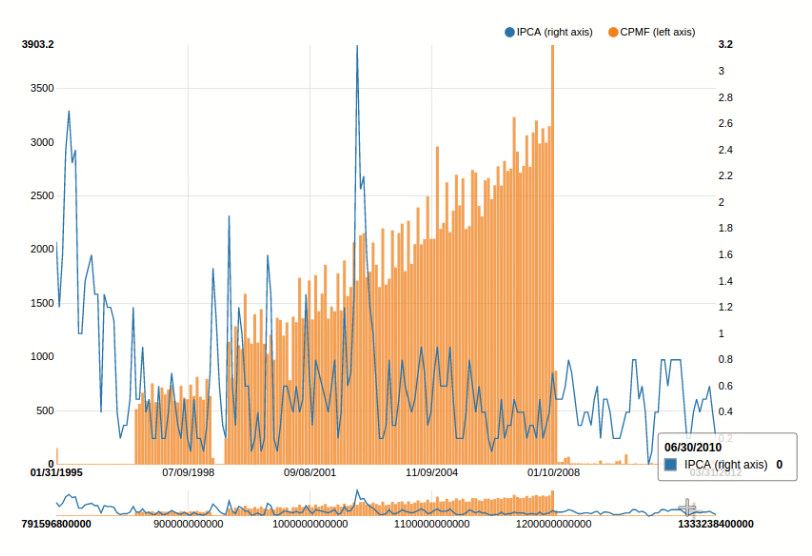
\includegraphics[width=0.8\textwidth]{./04-figuras/visualizacao}
    \fonte{O Autor}
    \label{fig:visualizacao}
\end{figure}

A fase de execução do teste de usabilidade do WOB contou com a participação de 6 usuários. 
Desses, 5 possuem formação na área de computação (Engenharia de Computação ou Sistemas de 
Informação), o último possui formação em Engenharia Mecânica, porém todos atuam na área de 
desenvolvimento de software. Além disso, 4 possuem alguma experiência com um dos temas: 
análise de dados, visualização de dados ou mineração de dados. É importante ressaltar que
essa quantidade de usuários se justifica, pois, segundo \citeonline{nielsen2000}, testes de 
usabilidade devem ser executados por 3 a 5 usuários.

Para cada um dos cenários propostos foram realizados testes com dois usuários diferentes. 
Para cada tarefa executada por um usuário, o avaliador considerava o tempo gasto em sua 
execução e, além disso, observava e anotava como a tarefa era concluída (i.e., concluída 
sem erro, concluída com erro ou não concluída). Não era permitido, ao longo da execução,
que o avaliador respondesse a perguntas referentes a interface, ou a alguma funcionalidade 
do WOB. Este tipo de pergunta seria respondida somente no período após cada tarefa, quando 
também seriam discutidas as dúvidas, dificuldades e sugestões dos usuários. 

Os testes de usabilidade, com os 6 usuários, ocorreram em um período de 3 dias, entre 27 de 
setembro de 2016 e 29 de setembro de 2016 sendo que cada um deles teve duração máxima de 
uma hora.

A partir dos dados obtidos, os resultados foram analisados de forma a caracterizar os 
indicadores de conclusão das tarefas pelos usuários; o tempo médio decorrido para cada uma 
das tarefas bem como o tempo médio total (i.e., tempo médio de conclusão de um cenário); e 
o grau de adequação do WOB aos princípios de usabilidade e colaboração. Através dessas 
medidas foi possível caracterizar a usabilidade e colaboração do WOB na perspectiva de 
seus usuários. Os resultados obtidos são discutidos a seguir.

\section{Discussão dos Resultados}
\label{sec:metodologia-resultados}

Em relação à execução das tarefas, o gráfico da Figura \ref{fig:avaliacao-tarefas} demonstra 
o percentual de conclusão de cada tarefa.

\begin{figure}[!htb]
    \centering
    \caption{Percentual de conclusão das tarefas pelos usuários}
    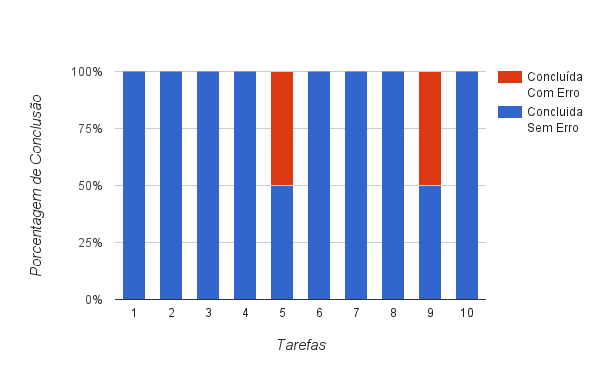
\includegraphics[width=0.8\textwidth]{./04-figuras/avaliacao-tarefas}
    \fonte{O Autor}
    \label{fig:avaliacao-tarefas}
\end{figure}

Através desse gráfico é possível observar que todas as tarefas foram concluídas pelos 
usuários, sendo que apenas 20\% foi concluída com erro, sendo a tarefa T5 concluída com 
erro por 2 usuários, e a tarefa T9 concluída com erro por 1 usuário.

A Tabela \ref{table:tempos-execucao}, por sua vez, apresenta o tempo decorrido para a execução 
de cada uma das tarefas pelos usuários e a média do tempo gasto pelos mesmos. Também são 
exibidos os tempos totais de execução das tarefas por cada usuário.

\begin{table}[!htb]
    \centering
    \caption{ Relação de tempo decorrido em minutos para cada uma das tarefas em cada teste de usabilidade}
    \label{table:tempos-execucao}
    \begin{tabular}{|p{1.2cm}|p{1.2cm}|p{1.2cm}|p{1.2cm}|p{1.2cm}|p{1.2cm}|p{1.2cm}|p{1.2cm}|p{1.5cm}|p{1.2cm}|}
        \hline
        &  \multicolumn{2}{p{2.4cm}|}{Cenário 1} & \multicolumn{2}{p{2.4cm}|}{Cenário 2} & \multicolumn{2}{p{2.4cm}|}{Cenário 3} & & &\\
        \hline
        Tarefa & U1 & U2 & U3 & U4 & U5 & U6 & Total de Usuários & Tempo Médio & Desvio Padrão \\
        \hline
        T1 & 01:07 & 03:09 & 01:56 & 01:20 & 00:00 & 00:00 & 4 & 01:53 & 00:55 \\
        \hline
        T2 & 00:18 & 00:31 & 00:27 & 00:20 & 00:00 & 00:00 & 4 & 00:24 & 00:06\\          
        \hline
        T3 & 01:18 & 00:40 & 00:29 & 00:15 & 00:00 & 00:00 & 4 & 00:40 & 00:27 \\
        \hline
        T4 & 01:22 & 01:01 & 00:51 & 01:38 & 00:00 & 00:00 & 4 & 01:13 & 00:21\\
        \hline
        T5 & 02:23 & 00:36 & 01:18 & 02:01 & 00:00 & 00:00 & 4 & 01:34 & 00:47\\
        \hline
        T6 & 02:06 & 00:41 & 02:07 & 00:57 & 00:00 & 00:00 & 4 & 01:27 & 00:45\\
        \hline
        T7 & 00:24 & 00:04 & 00:10 & 00:05 & 00:00 & 00:00 & 4 & 00:10 & 00:09\\
        \hline
        T8 & 00:52 & 00:35 & 01:13 & 01:29 & 01:11 & 00:54 & 6 & 01:02 & 00:19\\
        \hline
        T9 & 03:18 & 03:04 & 00:00 & 00:00 & 00:00 & 00:00 & 2 & 03:11 & 00:10\\
        \hline
        T10 & 00:00 & 00:00 & 03:35 & 03:52 & 04:33 & 04:13 & 4 & 04:03 & 00:25\\
        \hline 
        Total & 13:08 & 10:21 & 12:06 & 11:57 & 05:44 & 05:07 & - & - & -\\
        \hline   
    \end{tabular}
    \fonte{O Autor}
\end{table}


Os usuários U1 e U2 executaram o cenário C1, enquanto os usuários U3 e U4 executaram o 
cenário C2 e os usuários U5 e U6 executaram o cenário C3. Assim, também foi possível calcular
o tempo médio por cenário. Verificou-se que C1 possui um tempo médio de execução de 11 
minutos e 44 segundos, enquanto o tempo médio para concluir C2 é 12 minutos e 01 segundo, 
já o tempo médio para concluir C3 foi de 05 minutos e 25 segundos.

A tarefa T1 apresentou um tempo de execução similar entre a maioria dos usuários. Essa tarefa 
envolve acessar a página de instruções da ferramenta, para aprender sobre seu funcionamento. 
Embora essa tarefa não tenha gerado dificuldades ou dúvidas, foi possível perceber que a 
maioria dos usuários prefere aprender a utilizar a ferramenta durante a própria execução. 
Isso explica o tempo discrepante que ocorreu, pois um usuário se mostrou mais interessado 
em entender as instruções de como utilizar a ferramenta antes de utilizá-la de fato. Já a 
tarefa T2 foi executada sem maiores problemas e sem grande variação de tempo entre os 
usuários.

A tarefa T3 apresentou uma pequena variação nos tempos de execução entre os usuários. 
Nessa tarefa os usuários deveriam verificar o conjunto de dados enviado a partir da 
funcionalidade “\textit{preview}”. Durante a avaliação, 3 usuários reportaram dificuldades em 
localizar essa funcionalidade e, além disso, apresentaram sugestões de melhorias para 
a visibilidade dessa função. Embora esse tenha sido considerado um problema cosmético, 
as sugestões apontadas pelos usuários serão implementadas na próxima versão do WOB.

Já na execução da tarefa T4 não existiu nenhuma dúvida ou dificuldade. Uma tarefa que 
apresentou grande variação entre os tempos de execução foi a T5, além disso ela foi 
concluída com erro por 2 usuários. Nessa tarefa os usuários deveriam inserir \textit{tags} para 
cada coluna do conjunto de dados enviado e renomear suas colunas. Os erros ocorreram por 
dois motivos: (1) não ficou claro a possibilidade de editar os nomes das colunas e a 
forma de fazer isso, e (2) no processo para se adicionar uma \textit{tag} é mostrada uma lista 
com \textit{tags} já utilizadas anteriormente, não ficou claro, segundo os usuários, que era 
possível adicionar uma nova \textit{tag} que não existia nessa lista. Esse problemas serão 
corrigidos em versões futuras da ferramenta para melhorar a usabilidade do sistema.

A tarefa T6, embora tenha sido concluída sem erros por todos usuários, também apresentou 
problemas, o que fica claro com a variação entre os tempos de execução. Nessa tarefa 
deveria ser especificada uma hierarquia de dados dentro do conjunto de dados enviado. 
Dois usuários reportaram a falta de \textit{feedback} ao se definir a hierarquia, ou seja, não era 
possível saber se a hierarquia havia sido salva ou não. Esse problema também será corrigido 
em uma futura versão da ferramenta.

Na execução das tarefas T7, T8 e T10 não ocorreram problemas. Já a tarefa T9 foi concluída 
com erro por um usuário. Nessa tarefa os usuários deveriam utilizar a API disponível para 
recuperar o conjunto de dados enviado, e a partir disso gerar uma visualização. Uma possível 
explicação, para o erro cometido nessa tarefa, é a falta de experiência do usuário na 
utilização de \textit{web services}. Vale ressaltar que, embora o objetivo da ferramenta 
seja permitir sua utilização, mesmo por parte de usuários inexperientes, o projeto prevê uma 
segunda fase na qual será desenvolvida uma ferramenta de visualização de dados que irá 
consumir a API desenvolvida. Logo, isso não deverá ser um problema para usuários menos 
experientes no futuro, pois o acesso direto a API não será necessário.

Conforme mencionado anteriormente, depois de executadas as tarefas, cada usuário avaliou a 
ferramenta sob a perspectiva dos 07 princípios de usabilidade \cite{nielsen1994usability}, 
além dos 02 princípios de colaboração definidos especificamente para essa ferramenta, são 
eles: (1) colaboração passiva e (2) colaboração ativa.

O termo colaboração passiva se refere a utilizar um conjunto de dados já existente, ou 
seja, o grau com que o sistema permite que usuários utilizem conjuntos de dados que foram 
enviados por outros usuários, já o termo colaboração ativa se refere a enviar um conjunto 
de dados para outra pessoa utilizar, ou seja, o grau com que o sistema incentiva a 
colaboração entre usuários, mostrando que ao enviar um conjunto de dados ele estará 
disponível para qualquer um utilizar. O Quadro \ref{quadro:principios} sumariza os 07 princípios
de usablidade e os 02 princípios de colaboração.

\begin{quadro}[]
\centering
\caption{Princípios de Usabilidade e Colaboração}
\label{quadro:principios}
\begin{tabular}{|p{2cm}|p{13cm}|}
\hline
Princípio                 & Descrição                                                                                                                                                                                                                                                                \\ \hline
Facilidade de Aprendizado & \begin{tabular}[c]{@{}l@{}}Se refere ao tempo e esforço necessários para que os usuários aprendam \\ a utilizar uma determinada porção do sistema com bom nível de \\ competência e desempenho.\end{tabular}                                                                \\ \hline
Facilidade de Uso         & \begin{tabular}[c]{@{}l@{}}Está relacionado não apenas com o esforço cognitivo para interagir com \\ o sistema, mas também com a facilidade de completar a interação sem \\cometer erros durante este processo.\end{tabular}                                               \\ \hline
Flexível                  & \begin{tabular}[c]{@{}l@{}}Considera o quanto um sistema é capaz de acomodar caminhos distintos \\ para se atingir um mesmo objetivo, apoiando assim as preferências e \\modo de trabalho individuais dos usuários.\end{tabular}                                           \\ \hline
Produtivo                 & \begin{tabular}[c]{@{}l@{}}Analisa se o sistema consegue fazer bem aquilo a que se destina, e se o \\ usuário completa suas tarefas de  forma rápida e eficaz.\end{tabular}                                                                                               \\ \hline
Satisfatório              & \begin{tabular}[c]{@{}l@{}}Enfatiza a avaliação subjetiva do sistema feita pelo usuário, incluindo suas \\ preferências pessoais e emoções (positivas ou negativas) que possam \\surgir durante a interação.\end{tabular}                                                  \\ \hline
Útil                      & Relativo ao conjunto de funcionalidades oferecidas ao sistema para que os usuários realizem suas tarefas.                                                                                                                                                                \\ \hline
Seguro                    & \begin{tabular}[c]{@{}l@{}}Se refere ao grau de proteção de um sistema contra condições desfavorá-\\veis ou até mesmo perigosas para os usuários, envolvendo desde \\aspectos de recuperação de condições de erro até impacto no seu \\ trabalho ou sua saúde.\end{tabular} \\ \hline
Colaboração Ativa         & \begin{tabular}[c]{@{}l@{}}Se refere ao grau com que o sistema incentiva a colaboração entre usuá-\\rios, mostrando que ao enviar um conjunto de dados eles estará \\disponível para qualquer um utilizar.\end{tabular}                                                    \\ \hline
Colaboração Passiva       & \begin{tabular}[c]{@{}l@{}}Se refere ao grau com que o sistema permite que usuários utilizem \\ conjuntos de dados que foram enviados por outros usuários.\end{tabular}                                                                                                  \\ \hline
\end{tabular}
\end{quadro} 

Para que seja realizada uma análise mais assertiva, as respostas foram separadas de acordo 
com o cenário para o qual cada usuário foi submetido, dessa forma a 
Figura \ref{fig:avaliacao-cenario1} sumariza as respostas para os usuários que realizaram o 
cenário C1, a Figura \ref{fig:avaliacao-cenario2} para os usuários que realizaram o 
cenário C2 e a Figura \ref{fig:avaliacao-cenario3} para os usuários que realizaram o 
cenário C3.

\begin{figure}[!htb]
    \centering
    \caption{Grau de adequação do WOB por princípio de usabilidade e colaboração na visão dos usuários - Cenário C1}
    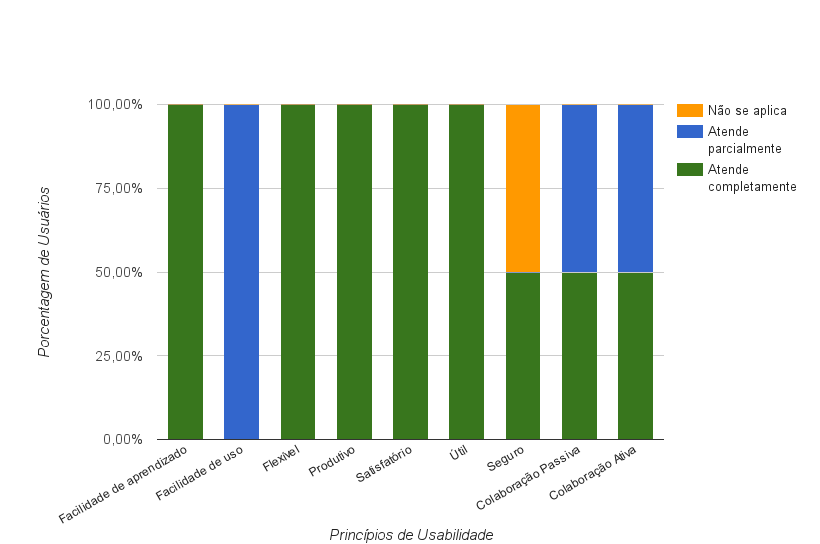
\includegraphics[width=0.87\textwidth]{./04-figuras/avaliacao-cenario1}
    \fonte{O Autor}
    \label{fig:avaliacao-cenario1}
\end{figure}

\begin{figure}[!htb]
    \centering
    \caption{Grau de adequação do WOB por princípio de usabilidade e colaboração na visão dos usuários - Cenário C2}
    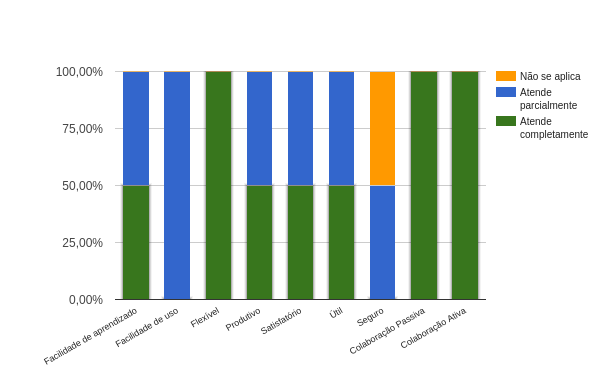
\includegraphics[width=0.87\textwidth]{./04-figuras/avaliacao-cenario2}
    \fonte{O Autor}
    \label{fig:avaliacao-cenario2}
\end{figure} 

\begin{figure}[!htb]
    \centering
    \caption{Grau de adequação do WOB por princípio de usabilidade e colaboração na visão dos usuários - Cenário C3}
    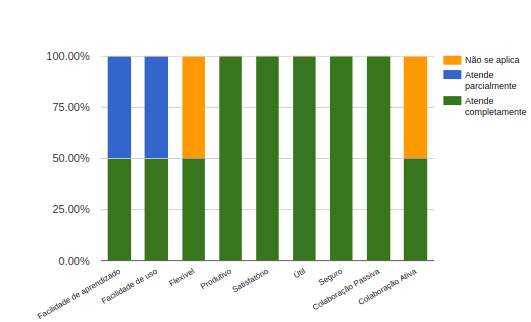
\includegraphics[width=0.9\textwidth]{./04-figuras/avaliacao-cenario3}
    \fonte{O Autor}
    \label{fig:avaliacao-cenario3}
\end{figure}


Através dos dados apresentados é possível observar que, nos três cenários, nenhum princípio 
foi julgado como “não atende”, na perspectiva dos usuários, ou seja, para todos os usuários 
todos os princípios são atendidos ou não são aplicáveis. Foi possível perceber que para 
66.67\% dos usuários o WOB atende completamente o princípio de facilidade de aprendizado, no 
entanto, para apenas 16.67\% o princípio de facilidade de uso é atendido completamente. Isso 
mostra que na visão desses usuários, embora, inicialmente, o WOB não apresente uma fácil 
utilização, aprender como utilizá-lo é uma tarefa simples. 

Pode-se notar também, que três princípios foram julgados como não aplicáveis. No cenário 
C1 e C2 foi o princípio “Seguro”, já no cenário C3 foram os princípios “Flexível” e 
“Colaboração Ativa”. Os usuários julgaram que o princípio “Seguro” não se aplica pois a 
ferramenta é aberta, permitindo sua utilização por qualquer pessoa. Já para os casos dos 
princípios “Flexível” e “Colaboração Ativa” os usuários julgaram que estes não se aplicam 
devido ao cenário que foram expostos. O cenário C3 envolve apenas a busca por dois 
conjuntos de dados já existentes no repositório e a utilização da API para o cruzamento 
desses dados, não envolvendo, portanto, caminhos alternativos ou o envio de conjuntos de 
dados para a utilização por outros usuários, isso explica a interpretação dos usuários 
ao responderem que os princípios não se aplicam.

Embora existam melhorias a serem implementadas, tanto que foram identificadas durante o 
teste, quanto aquelas que já estavam planejadas para futuras versões (ver lista de 
melhorias no Apêndice \ref{apendiceB}), conclui-se que a ferramenta WOB é adequada ao uso. 
Isso é corroborado pela fala dos usuários ao longo dos testes, que aprovaram a idéia por trás
da ferramenta bem como seu fluxo de execução. O capítulo seguinte conclui este trabalho, e 
propõe trabalhos futuros, a serem realizados, a partir do que foi desenvolvido até aqui.
                 % Avaliação
% -----------------------------------------------------------------------------
% Conclusão
% -----------------------------------------------------------------------------

\chapter{Conclusão}
\label{chap:conclusao}

% -----------------------------------------------------------------------------
% OBS: a norma ABNT estabelece que em qualquer tipo de trabalho acadêmico monográfico
% deve haver um capítulo de conclusão
% -----------------------------------------------------------------------------
                 % Conclusão

% Insere os elementos pós-textuais
\postextual
% -----------------------------------------------------------------------------
% Referências
% -----------------------------------------------------------------------------

% -----------------------------------------------------------------------------
% Carrega o arquivo "base-referencias.bib" e extrai automaticamente as referências citadas
% -----------------------------------------------------------------------------

\bibliography{./base-referencias}{}
\bibliographystyle{abntex2-alf} % Define o estilo ABNT para formatar a lista de referências

% -----------------------------------------------------------------------------
% Este arquivo não necessita de ser editado.
% -----------------------------------------------------------------------------
           % Referências
%% -----------------------------------------------------------------------------
% Apêndices
% -----------------------------------------------------------------------------

\begin{apendicesenv}
\partapendices

% -----------------------------------------------------------------------------
% Primeiro apêndice
% -----------------------------------------------------------------------------


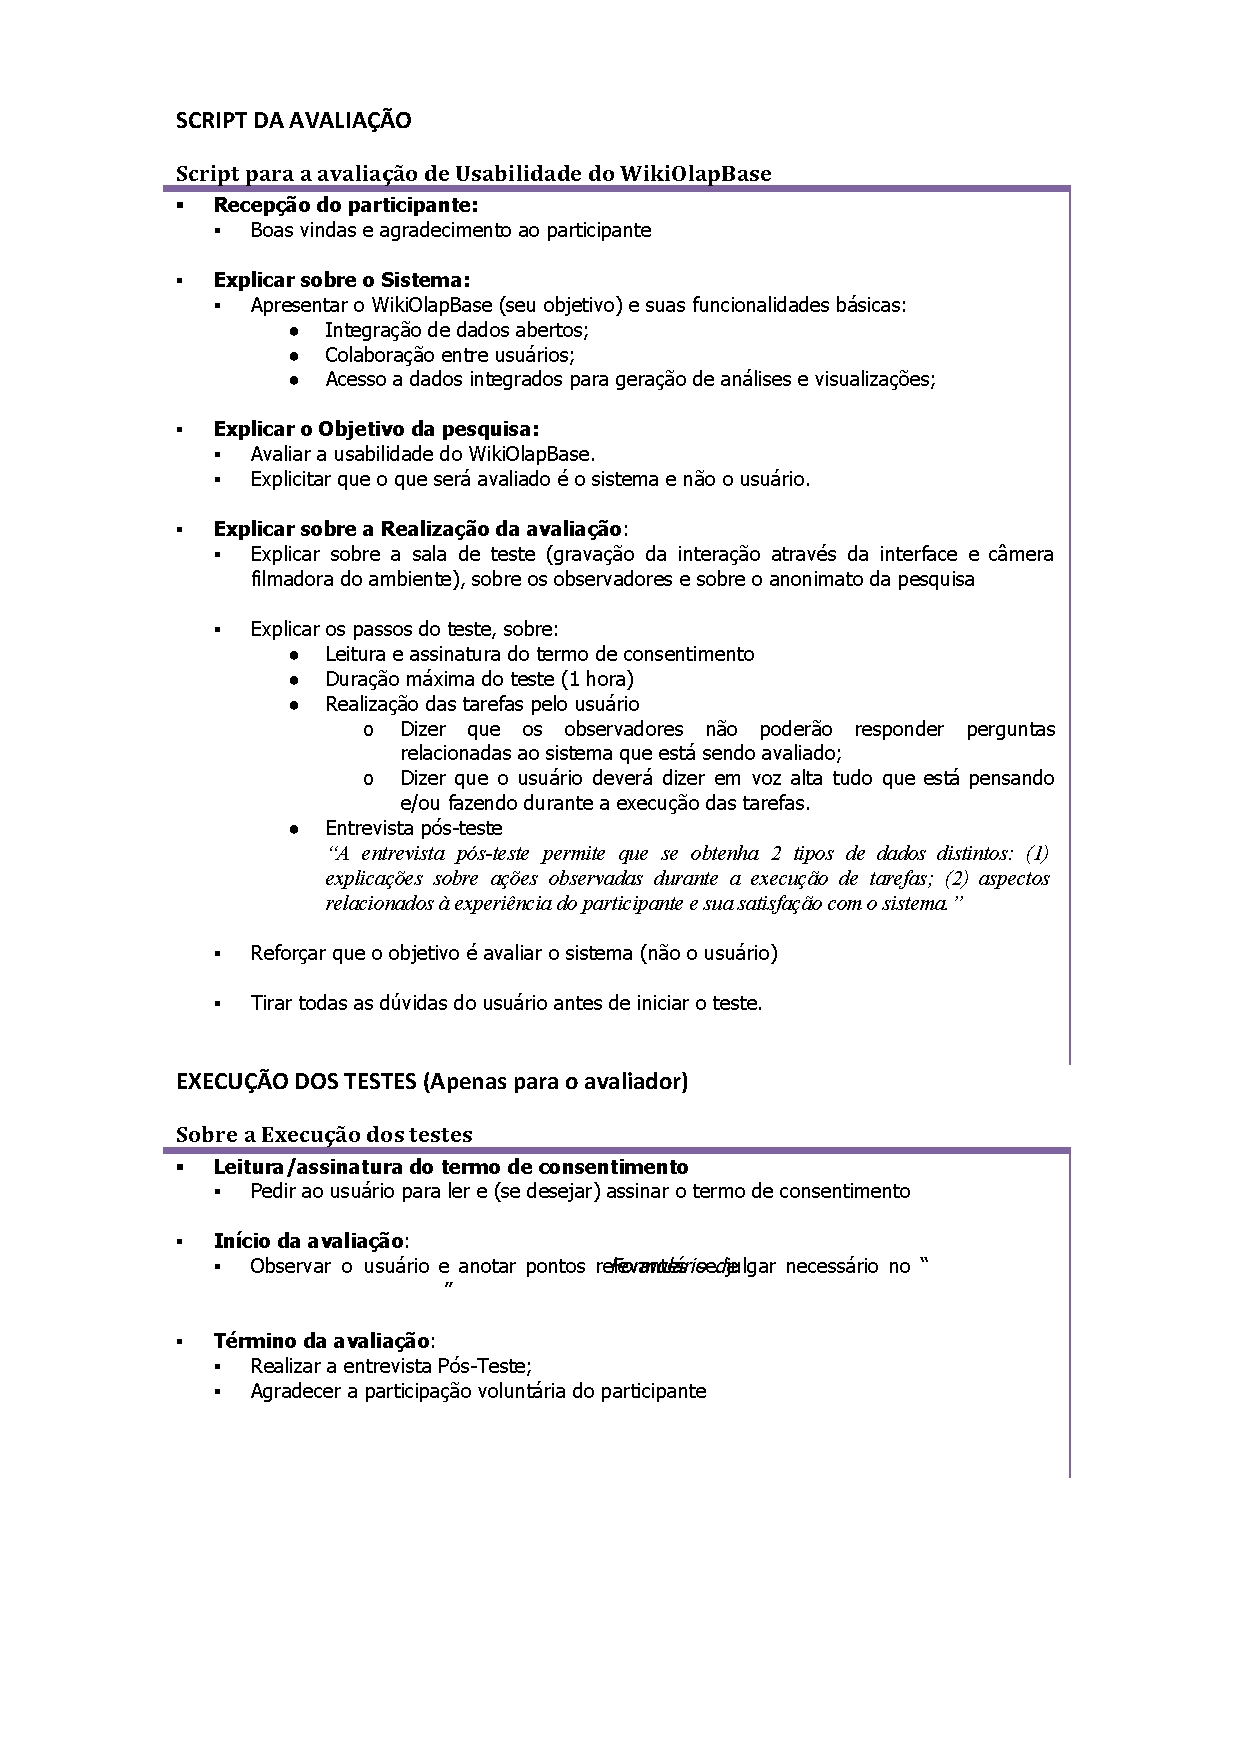
\includepdf[pages=1, scale=0.8,pagecommand=\chapter{Artefatos de Avaliação}\label{apendiceA}]{./04-figuras/avaliacao-artefatos}
\includepdf[pages=2-, scale=0.8, pagecommand={}]{./04-figuras/avaliacao-artefatos}

\chapter{Lista de Melhorias}
\label{apendiceB}

\begin{enumerate}  
    \item Criação de um sistema de cadastro e autenticação de usuários. 
    \item Adicionar suporte a outros formatos de arquivos. 
    \item Permitir o envio de arquivos compactados.
    \item Permitir o envio de múltiplos arquivos.
    \item Estender a função de busca para mostrar todos metadados.
    \item Incluir ícone na interface de editar nome das colunas para especificar a possibilidade de edição.
    \item Estender as funcionalidades da API para permitir outras operações e aplicação de filtros.
    \item Utilização de URIs para identifação das \textit{tags} das colunas. Utilizar, por exemplo, o schema.org.
\end{enumerate}

\end{apendicesenv}
             % Apêndices
%% -----------------------------------------------------------------------------
% Anexos
% -----------------------------------------------------------------------------

\begin{anexosenv}
\partanexos

% -----------------------------------------------------------------------------
% Primeiro anexo
% -----------------------------------------------------------------------------

\chapter{Nome do anexo}     % edite para alterar o título deste anexo
\label{chap:anexoA}


\end{anexosenv}
                % Anexos
%% -----------------------------------------------------------------------------
% Índice Remissivo
% -----------------------------------------------------------------------------

% -----------------------------------------------------------------------------
% Este comando gera automaticamente o índice remissivo para os termos definidos
% no corpo do documento
% -----------------------------------------------------------------------------

\printindex

% -----------------------------------------------------------------------------
% Este arquivo não necessita de ser editado.
% -----------------------------------------------------------------------------
      % Índice Remissivo

\end{document}
